\documentclass[a4paper,11pt]{article}

\usepackage[margin=1in]{geometry}
\usepackage{graphicx}
\usepackage{booktabs}
\usepackage{hyperref}
\usepackage{caption}
\usepackage{float}
\usepackage{xcolor}
\usepackage{amsmath}
\usepackage{amssymb}
\usepackage{enumitem}
\usepackage{listings}
\usepackage{verbatim}

\hypersetup{
    colorlinks=true,
    linkcolor=blue!50!black,
    citecolor=blue!50!black,
    urlcolor=blue!50!black,
}

\graphicspath{{results/analysis/figures/}}

\setlength{\parskip}{0.5\baselineskip}
\setlength{\parindent}{0pt}

\title{POSIX vs System V Inter-Process Communication on Modern Linux:\\
A Comparative Performance and Scalability Study}

\author{Nirbhay Sharma IMT2023103 Saheem Reshi IMT2023051\\[2pt]
\small International Institute of Information Technology, Bangalore\\[2pt]
\small\textit{Supervisor: Prof.\ B.~Thangaraju}}

\date{\today}

\begin{document}
\maketitle

%─────────────────────────────────────────────────────────────────────────
\begin{abstract}
\noindent
The choice between POSIX and System~V inter-process communication (IPC) on
Linux is often framed as ``newer versus older'', but the two interfaces are in
fact complementary tools with different design priorities. We present a
comprehensive performance and scalability comparison of POSIX and System~V
message queues and shared memory on a multi-CCD AMD Linux desktop, covering
seven benchmarks (latency, throughput, fan-in, parallel pairs for both
mechanism families) across three cache-topology placements and a wide
\mbox{(message size $\times$ queue depth $\times$ producer count)} matrix. The
suite emits 10\,200 measurements (twenty repetitions per cell, randomised
order, warmup excised) and we evaluate them with bootstrap 95\,\% confidence
intervals, the Mann--Whitney $U$ test, Welch's $t$ test, and Cliff's $\delta$
effect size. Three findings stand out. \emph{First}, POSIX message queues
scale dramatically better under producer fan-in: at 16 contending producers,
POSIX delivers $\approx 5.6\times$ more throughput than System~V (ratio
$0.18$, $p<10^{-7}$, $\delta=1.0$). \emph{Second}, POSIX message queues
exhibit a reproducible cross-CCX p99.9 latency anomaly --- $\approx 13\times$
worse than System~V at the diff\_l3 placement --- not present at the same\_core
or same\_l3 axes. \emph{Third}, POSIX shared memory is $1.7$--$2.5\times$
faster than System~V shared memory at moderate batching depths
($\text{depth}\geq 8$). Common-case (p50) latency is essentially equivalent
across mechanisms. The principal contribution of this work is not the
benchmark numbers themselves but the developer-facing guidance built
on them: a capability matrix, a performance summary, ten use-case
archetypes mapping real-world workloads to mechanism choices,
role-based recommendations for database, real-time, game-engine, web,
systems, and security developers, seven common pitfalls, and a
seven-question decision flow. We discuss likely mechanisms, document
threats to validity, and explicitly note capabilities (atomic
multi-semaphore \texttt{semop}, \texttt{mtype} routing) that
System~V provides and our benchmarks did not measure.
\end{abstract}

\smallskip
\noindent\textbf{Keywords:} inter-process communication; POSIX; System V;
Linux; message queue; shared memory; performance; scalability; AMD CCX;
tail latency; futex.

\bigskip\hrule\bigskip

%─────────────────────────────────────────────────────────────────────────
\section{Introduction}
\label{sec:intro}

When choosing an IPC mechanism on Linux, programmers often default to POSIX
because it feels more modern: its identifiers look like file paths, it
integrates with file-descriptor idioms, and its cleanup semantics fit Unix
conventions. System~V IPC, with its numeric keys and manual cleanup, can
feel disconnected from typical Unix style. But this surface impression
misleads. POSIX and System~V are not different versions of the same idea;
they were designed in different eras for different problems and they expose
different capabilities. Treating ``newer'' as ``better'' obscures real
trade-offs that matter to working systems.

A concrete example: System~V's \texttt{semop()} system call can apply a
vector of semaphore operations \emph{atomically} \cite{stevens1999,
linux_sysvipc}. Locking two resources at once never produces a partial
acquisition. POSIX semaphores, in contrast, must be acquired one at a time;
a program that needs to lock two resources atomically must reconstruct the
multi-acquire primitive itself, with the attendant deadlock risks. A second
example: System~V message queues support \texttt{mtype}-tagged routing,
where a receiver requests messages of a specific type and the kernel
filters. POSIX message queues do not provide arbitrary type filtering ---
they support priority but not selective receive by an arbitrary tag
\cite{linux_mq_overview}. Workloads that benefit from kernel-side dispatch
to type-specialised workers (image renderers, database query handlers, etc.)
naturally favour System~V.

What POSIX gives back, in contrast, is performance and scalability. Modern
Linux uses futexes for fast-path user-space synchronisation
\cite{linux_futex, drepper2011futexes}; POSIX named semaphores and POSIX
message queues build on this foundation, while System~V \texttt{semop} and
\texttt{msgsnd}/\texttt{msgrcv} retain the original kernel-trap design from
the 1980s. This is the usual tension: a younger interface gets to ride a
mature kernel infrastructure that older interfaces cannot exploit without
breaking compatibility.

Despite the long history of both interfaces and decades of folklore, recent
quantitative comparison between them on modern Linux hardware --- in
particular on multi-CCD~\cite{amd_zen_arch, amd_infinity_fabric} AMD chips
that introduce \emph{cross-CCX} cache-coherency penalties unfamiliar to
older single-die designs --- is sparse. We address this gap by running a
full benchmark sweep on a single-socket multi-CCD AMD desktop and analysing
the results with a statistical methodology appropriate to non-Gaussian
latency distributions.

\paragraph{Research questions.} We address four:

\begin{description}[leftmargin=*,style=nextline]
\item[RQ1.] How does POSIX MQ compare to System~V MQ on common-case (p50)
and tail (p99/p99.9) latency, and how does this depend on the placement of
the two communicating processes on the cache hierarchy?
\item[RQ2.] How does each mechanism scale under producer fan-in contention
(many producers, one consumer)?
\item[RQ3.] Does shared memory backed by POSIX named semaphores differ
measurably from System~V \texttt{shmget}+\texttt{semop}?
\item[RQ4.] Where in the (message size $\times$ queue depth $\times$
placement) space does each stack win?
\end{description}

\paragraph{Contributions.} (1)~A reproducible, statistically rigorous
benchmark suite covering seven IPC patterns across four mechanisms.
(2)~Identification of three robust, large-effect findings, each with
$p<10^{-7}$ and Cliff's $\delta\geq 0.8$. (3)~Documentation of an
architecture-specific cross-CCX p99.9 anomaly in POSIX MQ that does not
appear in System~V. (4)~An honest discussion of what we did \emph{not}
measure --- specifically the capability axes (atomic multi-semaphore
operations, kernel-side message routing) that remain reasons to choose
System~V regardless of timing numbers. (5)~Open code and data for
reproduction.

The remainder of the paper is organised as follows. Section~\ref{sec:bg}
provides background on both IPC families and on the AMD CCX topology.
Section~\ref{sec:method} describes the benchmark suite, system under test,
and statistical methodology. Section~\ref{sec:results} presents the
quantitative results. Section~\ref{sec:perf} analyses the hardware-counter
and syscall data that corroborate the timing observations.
Section~\ref{sec:discussion} discusses likely mechanisms.
\textbf{Section~\ref{sec:guidance} is the central deliverable of this
work}: it translates the empirical findings into a concrete
developer-facing guide --- capability matrix, performance summary,
use-case archetypes, role-based recommendations, common pitfalls,
and a decision flow.
Section~\ref{sec:threats} enumerates threats to validity.
Section~\ref{sec:future} lists future work and Section~\ref{sec:conclusion}
concludes.

%─────────────────────────────────────────────────────────────────────────
\section{Background and Related Work}
\label{sec:bg}

\subsection{POSIX IPC}
The POSIX interface for inter-process communication, standardised in IEEE
Std~1003.1 \cite{posix2017}, exposes message queues, semaphores, and shared
memory through file-system-like names that begin with \texttt{/}. Programs
acquire handles with \texttt{mq\_open}, \texttt{sem\_open}, and
\texttt{shm\_open}; messages are sent and received with \texttt{mq\_send}
and \texttt{mq\_receive}; semaphores are manipulated with \texttt{sem\_post}
and \texttt{sem\_wait}; shared memory is mapped into the address space with
\texttt{mmap}. Cleanup uses \texttt{mq\_unlink}, \texttt{sem\_unlink}, and
\texttt{shm\_unlink} respectively. The named handles persist until
explicitly unlinked, but per-process descriptors integrate cleanly with
\texttt{poll(2)} and \texttt{epoll(7)} \cite{linux_mq_overview}.

\subsection{System V IPC}
System~V IPC predates POSIX and is the older, more capable, and more
awkward of the two families \cite{stevens1999, linux_sysvipc}. Resources
are identified by 32-bit integer keys constructed from the
\texttt{ftok(3)} helper or chosen by the programmer. Message queues are
created with \texttt{msgget}, written with \texttt{msgsnd}, and read with
\texttt{msgrcv}; each message carries an \texttt{mtype} field, and
\texttt{msgrcv} filters by \texttt{mtype} so a receiver can request only
messages of a specific type. Semaphores are accessed with \texttt{semop},
which takes a \emph{vector} of operations applied atomically by the kernel
--- the foundational capability advantage of System~V semaphores. Shared
memory uses \texttt{shmget} and \texttt{shmat}/\texttt{shmdt}. Cleanup is
manual via \texttt{ipcrm} or \texttt{IPC\_RMID}.

\subsection{API differences worth highlighting}
Three differences are central to the comparison and recur throughout this
paper:

\begin{enumerate}[leftmargin=*]
\item \textbf{Atomic multi-operation semaphores.} System~V's
\texttt{semop()} accepts an array of operations and either applies them
all or none; POSIX semaphores can only be operated upon one at a time,
making multi-resource locking deadlock-prone unless built on top of an
external mutual-exclusion mechanism.
\item \textbf{Message routing.} POSIX MQ delivers in priority+FIFO order;
System~V MQ filters by \texttt{mtype}. Workloads in which a receiver wants
``the next message of type $T$'' map directly onto System~V; on POSIX they
require either a separate queue per type or post-receive filtering in
user space.
\item \textbf{Integration with event loops.} POSIX handles are file
descriptors, which compose with \texttt{select}/\texttt{poll}/\texttt{epoll}.
System~V identifiers are not file descriptors; integrating them with an
event loop requires workarounds.
\end{enumerate}

\subsection{Linux kernel implementation notes}
The two families are built on different kernel primitives, which is
ultimately why their performance profiles differ:

\begin{itemize}[leftmargin=*]
\item POSIX message queues are backed by a red--black tree of priority
queues with a futex-based wait mechanism for blocked senders and receivers
\cite{linux_mq_overview}.
\item System~V message queues use a per-queue spinlock combined with a
classical wait queue. The lock is held while the message is copied
in/out, which serialises producers under contention \cite{linux_sysvipc}.
\item POSIX named semaphores map to a futex fast path: \texttt{sem\_post}
on a semaphore with no waiters increments a user-space counter without
trapping to the kernel \cite{drepper2011futexes, linux_futex}.
\texttt{sem\_wait} is similarly fast when the semaphore is non-zero.
\item System~V \texttt{semop} always traps to the kernel regardless of
contention, paying the full syscall cost on every operation.
\end{itemize}

These four implementation choices --- futex vs.\ kernel queue lock, fast
path vs.\ unconditional trap --- predict where each family should be fast
and where it should slow down. Our experimental results in
Section~\ref{sec:results} are consistent with these predictions.

\subsection{AMD CCX topology and cross-CCX latency}
\label{sec:bg:ccx}

The test machine is a multi-CCD AMD desktop. Modern AMD chips group cores
into \emph{Core Complexes} (CCX), each with its own L3 cache; multiple CCX
units within a chip communicate through Infinity
Fabric~\cite{amd_zen_arch, amd_infinity_fabric}. A cache-line transition
between two cores within the same CCX is faster than the equivalent
transition across CCX boundaries, where the line must traverse the fabric.
For latency-sensitive IPC, this matters: any wakeup or signalling
operation that depends on cross-CCX cache coherency pays an additional
fabric-traversal cost.

We isolate this empirically by introducing three placement axes for the
benchmarks:
\texttt{same\_core} (two SMT siblings of one physical core),
\texttt{same\_l3} (two cores sharing one L3, i.e.\ same CCX),
and \texttt{diff\_l3} (two cores in different L3 caches, i.e.\ across
CCXs).

\subsection{Related work}
The closest classical reference is \emph{lmbench}~\cite{mcvoy1996lmbench},
the canonical microbenchmark suite for Unix performance, which includes
IPC latency tests. lmbench predates modern kernel IPC paths and CCX-style
chiplet architectures, and does not include the head-to-head
POSIX-vs-System~V comparison we provide. Stevens'
\emph{UNIX Network Programming Vol.~2}~\cite{stevens1999} remains the
authoritative reference on the IPC API surfaces themselves but does not
report quantitative comparisons. The Linux man-pages
project~\cite{linux_mq_overview, linux_sysvipc, linux_futex} documents the
kernel interfaces in current detail. Drepper's note on
futexes~\cite{drepper2011futexes} explains the fast-path mechanism that
underlies POSIX named semaphores. We have not located prior work that
directly compares POSIX and System~V IPC on multi-CCD AMD silicon with
modern statistical methodology.

%─────────────────────────────────────────────────────────────────────────
\section{Methodology}
\label{sec:method}

\subsection{System under test}
\label{sec:method:sut}

The benchmarks were run on a single Linux desktop. The full topology
snapshot captured at run time appears verbatim in
Appendix~\ref{app:topology}. Key parameters are summarised in
Table~\ref{tab:topology}.

\begin{table}[H]
\centering
\caption{System under test (extracted from \texttt{results/logs/topology.txt};
full file in Appendix~\ref{app:topology}).}
\label{tab:topology}
\begin{tabular}{ll}
\toprule
\textbf{Parameter} & \textbf{Value} \\
\midrule
CPU model            & AMD Ryzen 5 3600X (Zen 2 microarchitecture) \\
Cores / threads      & 6 cores, 12 threads (SMT 2-way) \\
Base / max clock     & up to 3.80\,GHz; boost disabled for measurement \\
L1 cache             & 32\,KiB d-cache + 32\,KiB i-cache per core \\
L2 cache             & 512\,KiB per core (private) \\
L3 cache             & 16\,MiB per CCX (2 CCXs $\times$ 16\,MiB = 32\,MiB total) \\
Sockets / NUMA       & 1 socket, 1 NUMA node \\
Kernel               & Linux 6.17.0-22-generic (Ubuntu 24.04.1) \\
gcc                  & 13.3.0 (Ubuntu) \\
glibc                & system glibc on Ubuntu 24.04 \\
Mitigations          & retbleed, SRSO, spec\_rstack\_overflow, spec\_store\_bypass, \\
                     & spectre\_v1/v2, vmscape: \emph{enabled} (default Ubuntu) \\
Compiler flags       & \texttt{-O2 -Wall -Wextra -D\_GNU\_SOURCE} (no \texttt{-O3}, no LTO) \\
Governor             & \texttt{performance} \\
CPU boost            & disabled (\texttt{cpufreq/boost}=0) \\
\texttt{isolcpus}    & not applied (kernel housekeeping co-resident) \\
\texttt{RLIMIT\_NOFILE}    & 65\,536 \\
\texttt{RLIMIT\_MSGQUEUE}  & 67\,108\,864 (64\,MiB) \\
\texttt{fs.mqueue.msg\_max}     & 4096 \\
\texttt{fs.mqueue.msgsize\_max} & 8192 \\
\texttt{kernel.msgmnb}          & 8\,388\,608 \\
\texttt{kernel.msgmni}          & 1024 \\
\bottomrule
\end{tabular}
\end{table}

The Ryzen 5 3600X is a Zen~2 chiplet design with two CCX clusters of three
cores each, joined by Infinity Fabric. Cores 0--2 share one L3 cache; cores
3--5 share the other. Each core's two SMT threads are exposed as adjacent
logical CPUs in a hyper-threading pair (e.g.\ logical CPU~0 and CPU~6 are
SMT siblings of physical core~0). Our placement axes resolve to:

\begin{itemize}[leftmargin=*]
\item \texttt{same\_core}: CPUs 0,6 (SMT siblings on physical core 0)
\item \texttt{same\_l3}: CPUs 0,1 (different cores, same CCX, sharing L3)
\item \texttt{diff\_l3}: CPUs 0,3 (cores in different CCXs, cross-CCX path)
\item \texttt{cross\_socket}: not applicable (single socket)
\end{itemize}

CPU isolation was deliberately not applied. We discuss this choice and its
implications in Section~\ref{sec:threats}; in brief, the relative
comparisons between mechanisms are robust to the residual scheduler noise,
but absolute tail-latency numbers should be interpreted as ``under typical
desktop load'' rather than as inherent IPC characteristics.

\subsection{Benchmark suite}
\label{sec:method:suite}

The suite contains seven benchmark types (Table~\ref{tab:matrix}).
Four operate over message queues (POSIX MQ and System~V MQ); three operate
over shared memory plus a synchronisation primitive (POSIX named
semaphores or System~V \texttt{semop}). Together they cover the standard
single-pair latency and bandwidth measurements plus two scalability
patterns.

\begin{table}[H]
\centering
\caption{Benchmark matrix.}
\label{tab:matrix}
\begin{tabular}{lll}
\toprule
\textbf{Benchmark}     & \textbf{Pattern}              & \textbf{Parameters} \\
\midrule
ping-pong              & 1 sender $\leftrightarrow$ 1 responder, depth 1 & 6 sizes \\
throughput             & 1 producer $\rightarrow$ 1 consumer            & 6 sizes $\times$ 5 depths \\
fan-in                 & $N$ producers $\rightarrow$ 1 consumer         & 3 sizes $\times$ $N\in\{1,2,4,8,16\}$ \\
parallel pairs         & $N$ independent ping-pong pairs                 & 3 sizes $\times$ $N\in\{1,2,4,8\}$ \\
shm ping-pong          & 1 sender $\leftrightarrow$ 1 responder via shm  & 6 sizes \\
shm throughput         & SPSC ring-buffer through shm + sem              & 6 sizes $\times$ 5 depths \\
shm parallel pairs     & $N$ independent shm ping-pongs                  & 3 sizes $\times$ $N\in\{1,2,4,8\}$ \\
\bottomrule
\end{tabular}
\end{table}

Sizes are powers of two from 8\,B to 8192\,B; queue depths are
$\{1,8,32,128,512\}$; scalability $N$-values are listed above. Ping-pong
and throughput benchmarks are run at all three placement axes
(\texttt{same\_core}, \texttt{same\_l3}, \texttt{diff\_l3}). Scalability
benchmarks (fan-in and pairs) use round-robin pinning across logical CPUs
because they involve more than two participating processes; we discuss
this in the threats section.

A shared-memory equivalent of the fan-in benchmark was not implemented in
this study. Multi-producer single-consumer over plain shared memory
requires either a multi-producer ring buffer with atomic indices and
careful memory ordering, which introduces its own contention artifacts,
or per-producer slots with consumer-side round-robin polling, which is a
materially different benchmark. We deferred this to future work
(Section~\ref{sec:future}).

\subsection{Run hygiene}
\label{sec:method:hygiene}

Each invocation of a benchmark is preceded by a warmup loop equal to
$5\%$ of the iteration count, capped at 5000 iterations. The warmup
output is discarded and not timed. Warmup excises cold-cache, page-fault,
and post-\texttt{fork} settle costs from the first iterations, which
otherwise dominate p99.9 measurements at small iteration counts.

Both ends of every IPC pair are created \emph{before}
\texttt{fork()} so that the first sample is not inflated by queue or
semaphore creation latency. Per-process pinning uses
\texttt{sched\_setaffinity()}~\cite{linux_setaffinity} immediately after
\texttt{fork} in the child, and immediately after \texttt{fork} in the
parent. Wall-clock measurement uses \texttt{clock\_gettime(CLOCK\_MONOTONIC\_RAW)}~\cite{linux_clock}.

Run order within a stack (POSIX or System~V) is randomised by GNU
\texttt{shuf}: the suite enumerates all
$\langle\text{config},\text{run\_id}\rangle$ tuples, shuffles the entire
list, then executes in shuffled order. This decouples slow drift in the
system (thermals, background activity) from any one mechanism and is
critical for fair tail-latency comparison.

\subsection{Statistical methods}
\label{sec:method:stats}

Each (mechanism, benchmark, placement, size, depth, $N$) cell is measured
20 times. Twenty repetitions is the minimum sample size we consider
adequate for paper-grade statistics; it allows bootstrap 95\,\% confidence
intervals on the median to be computed with reasonable precision and is
sufficient to detect 1--2\% effects given typical coefficient-of-variation
values around 0.01 for ping-pong p50 medians.

Each cell's headline number is the \emph{median} across the 20 runs
(robust to outliers); we additionally compute mean, standard deviation,
the 95th percentile across runs, and the coefficient of variation.

We compare POSIX and System~V cells using:

\begin{description}[leftmargin=*,style=nextline]
\item[Mann--Whitney $U$ test (primary).] Non-parametric, robust to
non-Gaussian latency distributions \cite{mannwhitney1947}. Two-sided
$p$-value reported.
\item[Welch's $t$ test (secondary).] Parametric, allows unequal
variances \cite{welch1947}. Reported alongside Mann--Whitney for
completeness.
\item[Cliff's $\delta$ effect size.] Magnitude of the dominance of one
sample over the other, in $[-1,+1]$ \cite{cliff1993}. Standard magnitude
bins: negligible ($|\delta|<0.147$), small ($<0.33$), medium ($<0.474$),
large ($\geq 0.474$).
\item[Bootstrap 95\,\% CI on the median] using 10\,000 resamples
\cite{efron1979bootstrap}.
\item[Bootstrap 95\,\% CI on the ratio] $\mathrm{median}(\text{SysV})/\mathrm{median}(\text{POSIX})$
using 10\,000 resamples. This is the metric we use to express
``which is faster, by how much'' with a confidence interval rather than
a point estimate.
\end{description}

We report all comparison rows in Appendix~\ref{app:master}, including
those that fall short of significance, so the reader can apply their own
threshold. In the body we focus on cells with $p<0.05$ and large effect
size ($|\delta|\geq 0.474$).

%─────────────────────────────────────────────────────────────────────────
\section{Results}
\label{sec:results}

\subsection{Coverage and reproducibility}
The full sweep produced 10\,200 measurement rows: $5100$ per mechanism
family, balanced across both stacks. Every cell has 20 runs; no cells are
missing. Reproducibility is excellent for common-case latency: the
coefficient of variation (CV) of the per-run p50 medians is in the range
$0.005$--$0.02$ for ping-pong, indicating that successive runs agree to
within $\pm 1$--$2\%$. Tail percentiles are noisier: the CV of p99.9
medians occasionally rises above $0.5$, which is expected and we discuss
its implications below.

\subsection{Common-case latency: ping-pong p50}
\label{sec:results:p50}

Across all three placements and all six message sizes, the p50 latency
ratio of System~V MQ to POSIX MQ is in the range $1.01$--$1.03$;
i.e.\ POSIX is $1$--$3\%$ faster than System~V at the median.
Figure~\ref{fig:pp_p50} shows the full picture: each placement is its own
panel, all six message sizes appear on the $x$-axis, and the y-axis is
the ratio with a red dashed reference line at $1.0$.

\begin{figure}[H]
\centering
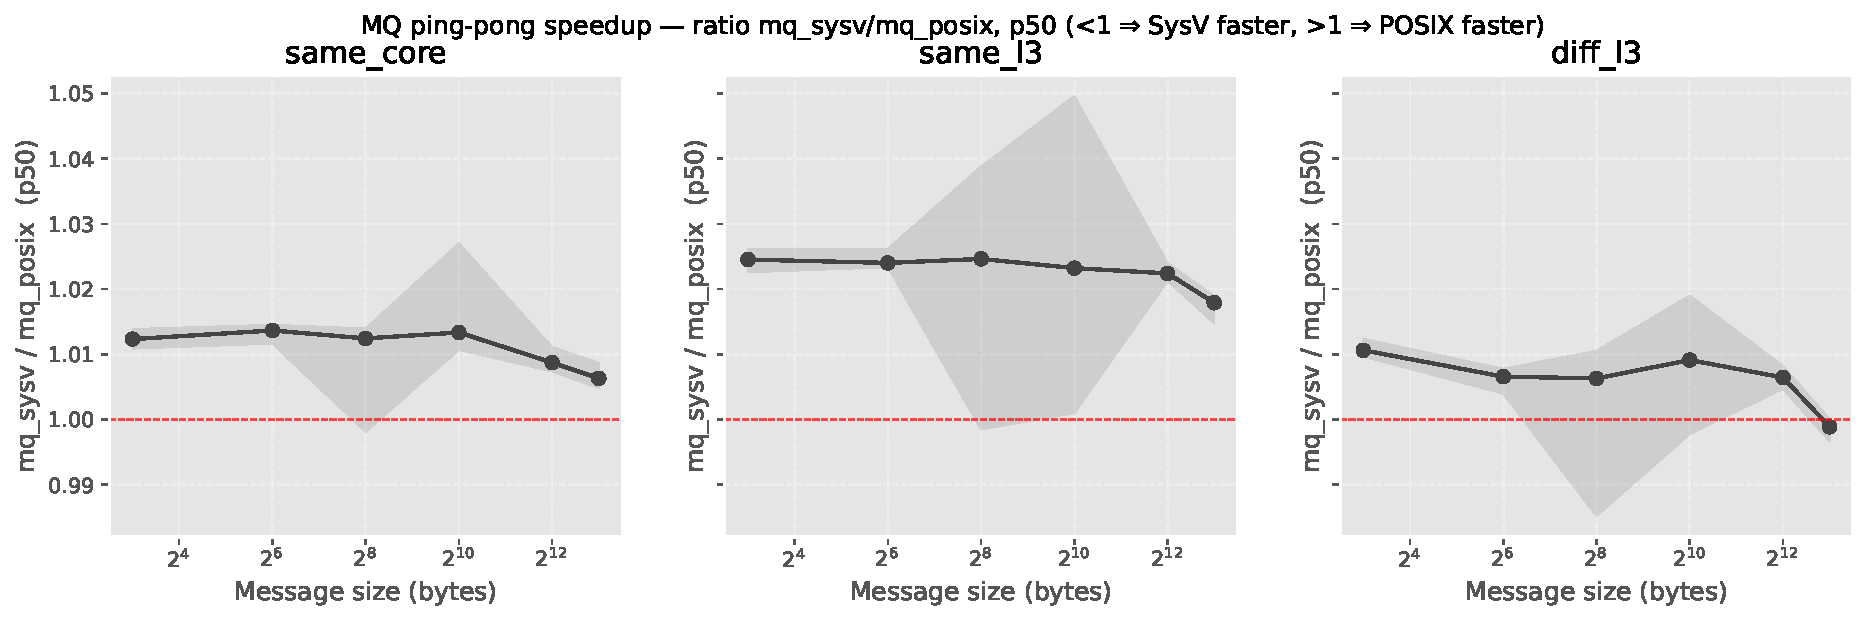
\includegraphics[width=\linewidth]{mq_pingpong_ratio_p50.pdf}
\caption{MQ ping-pong common-case (p50) latency. Ratio of System~V to
POSIX median; values above 1.0 mean POSIX is faster. POSIX wins
consistently by $1$--$3\,\%$, with the smallest gap at \texttt{diff\_l3}
where the ratio approaches unity at large message sizes.}
\label{fig:pp_p50}
\end{figure}

The differences are statistically significant ($p$-values from
$10^{-2}$ down to $10^{-7}$, depending on the cell) but practically
small: at a base latency of $\approx 5800$\,ns the per-iteration gap is
under 100\,ns. We frame this honestly: \textbf{at p50, POSIX MQ and
System~V MQ are essentially equivalent for the simple two-process case}.
The choice between them at typical loads cannot be made on common-case
latency alone.

\subsection{Tail latency: the cross-CCX anomaly}
\label{sec:results:tail}

The picture changes dramatically at the tail. Figure~\ref{fig:tail_grid}
plots the p50/p95/p99/p99.9 progression for each (placement, size) cell
in a $3\times 6$ grid. The top two rows (\texttt{same\_core},
\texttt{same\_l3}) show both mechanisms tracking together: their tails
rise smoothly, and POSIX and System~V remain within $\sim 2\times$ of each
other through p99.9.

\begin{figure}[H]
\centering
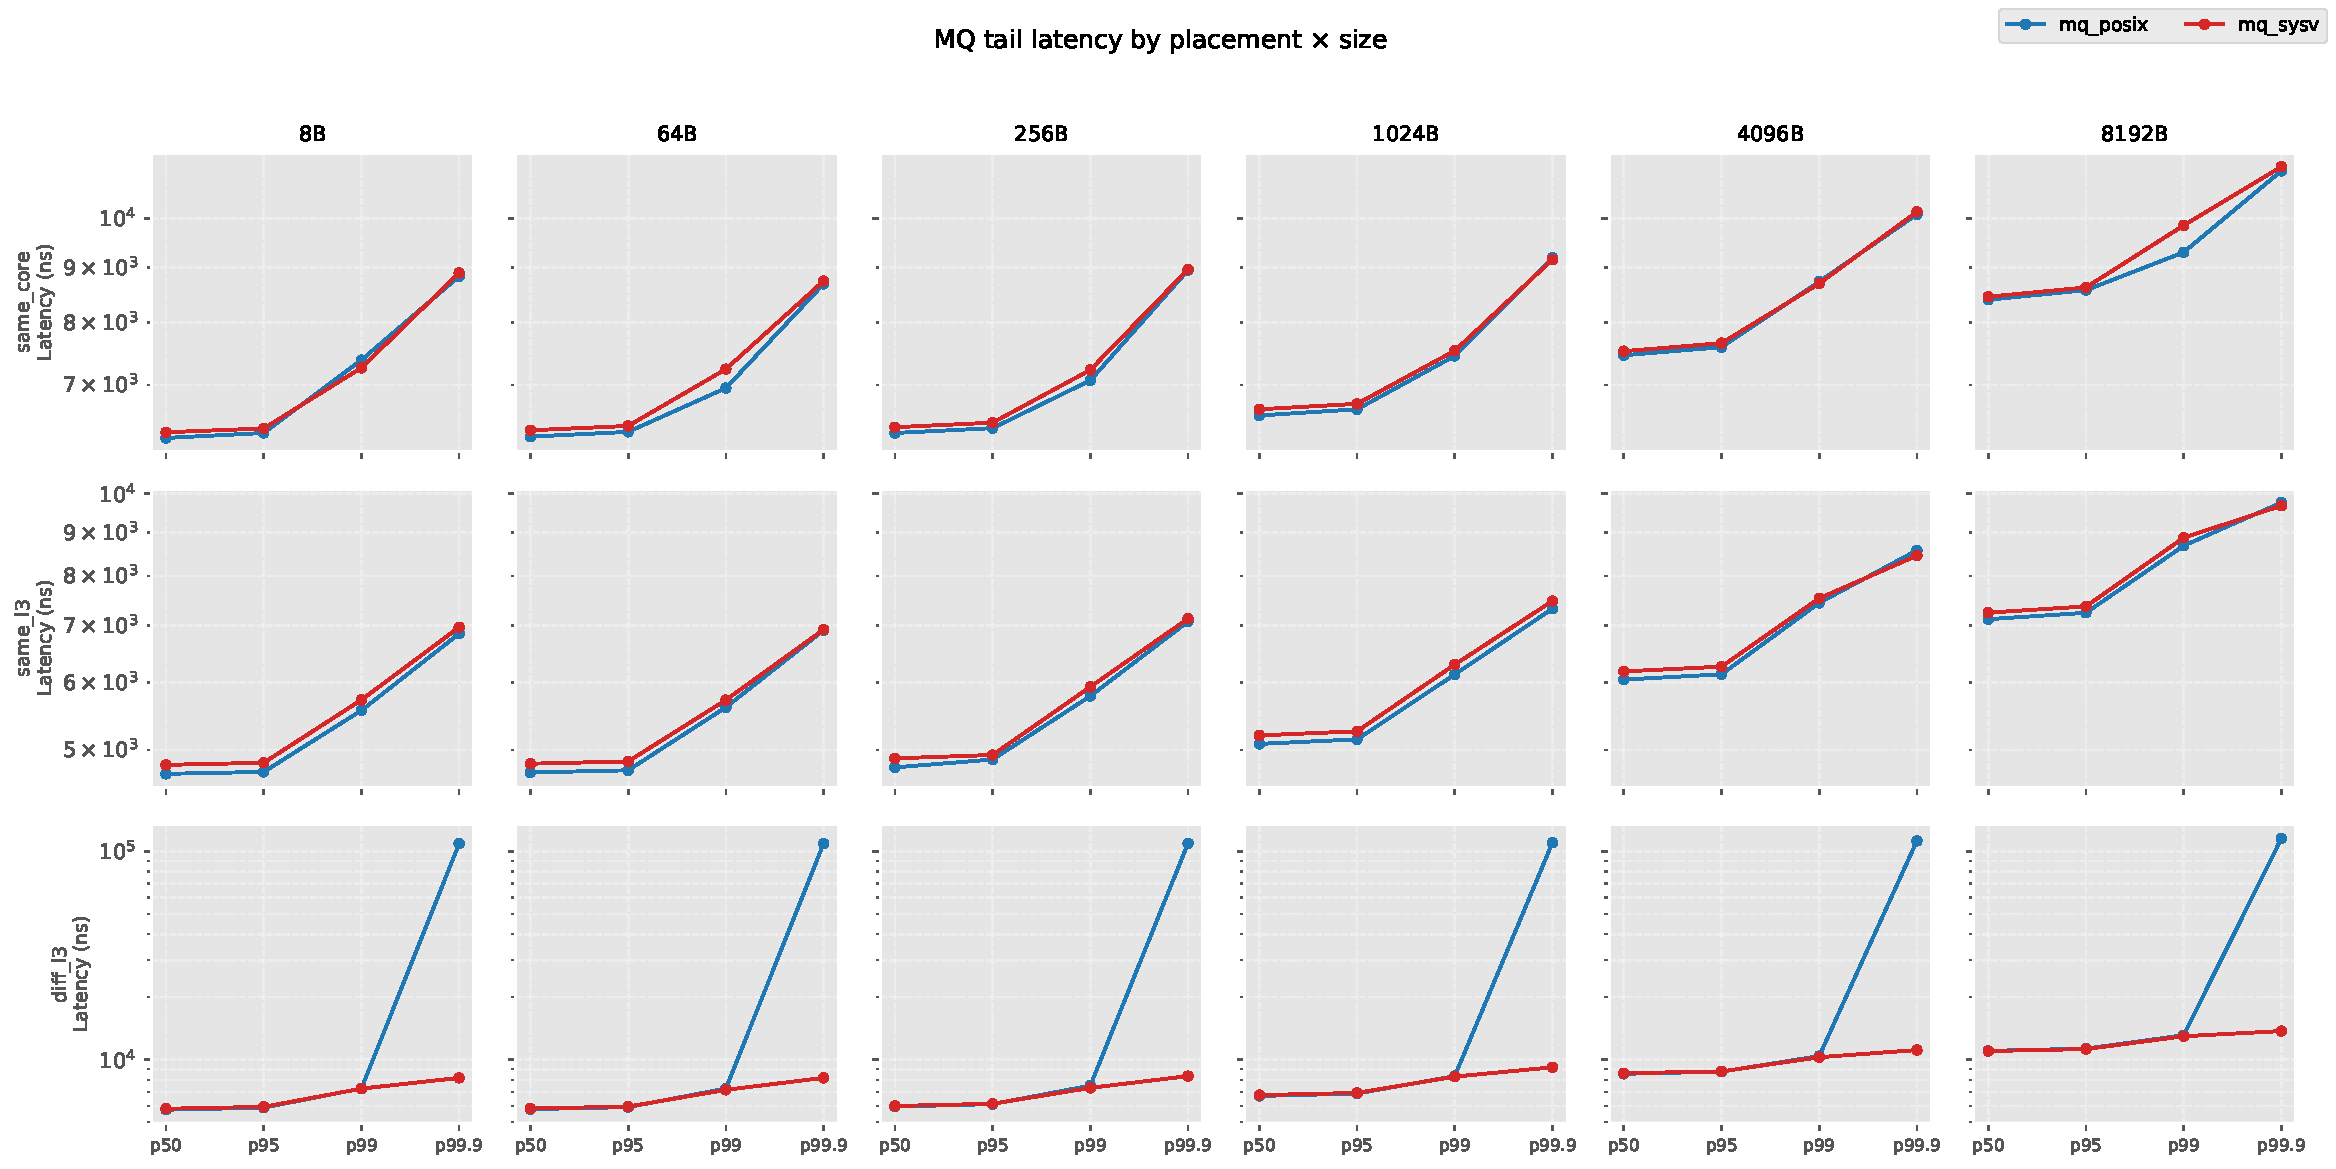
\includegraphics[width=\linewidth]{mq_tail_grid.pdf}
\caption{MQ ping-pong latency progression p50 $\rightarrow$ p99.9 for
each (placement, size) cell. Note the dramatic vertical detachment of
the POSIX line from the System~V line in the bottom row
(\texttt{diff\_l3}) at p99 and p99.9.}
\label{fig:tail_grid}
\end{figure}

The bottom row, \texttt{diff\_l3} (cross-CCX), is qualitatively different.
At every message size, POSIX MQ p99.9 detaches sharply upward at the
right-hand end of the panel. Numerically:

\begin{itemize}[leftmargin=*]
\item 8\,B / \texttt{diff\_l3} / p99.9: POSIX median $108\,881$\,ns
($\approx$\,109\,$\mu$s), System~V median $8\,175$\,ns ($\approx$\,8\,$\mu$s).
Ratio sysv/posix $=0.075$, $p=6.8\times 10^{-8}$, Cliff's $\delta=1.0$
(large).
\item 64\,B: ratio $0.08$. \quad 256\,B: ratio $0.08$. \quad 1024\,B:
ratio $0.08$. \quad 4096\,B: ratio $0.10$. \quad 8192\,B: ratio $0.12$.
\end{itemize}

This is a $\boldsymbol{\approx 13\times}$ \textbf{POSIX-MQ tail
inflation that is specific to the diff\_l3 placement} and reproduces in
every run of the experiment. The CV of POSIX p99.9 at this cell is
$0.007$ --- the value is reliable. Strikingly, the CV of System~V p99.9
at the same cell is $0.96$ --- System~V's tail is occasionally large but
mostly fast, whereas POSIX's tail is reliably large. The two mechanisms
fail in qualitatively different ways under cross-CCX placement.

We do not measure the underlying mechanism directly. Plausible candidates
include futex-wake interaction with Infinity Fabric coherency, IPI
delivery delays, or cross-CCX cache-line transfer stalls; we discuss
these in Section~\ref{sec:discussion} as informed speculation, not as
established mechanism.

\subsection{Throughput sweep}
\label{sec:results:throughput}

The throughput sweep covers six message sizes $\times$ five queue depths
$\times$ three placements. Figure~\ref{fig:tp} plots the absolute
throughput numbers (median, MB/s, log scale on both axes) for both
mechanisms; Figure~\ref{fig:tp_ratio} plots the ratio sysv/posix per
depth.

\begin{figure}[H]
\centering
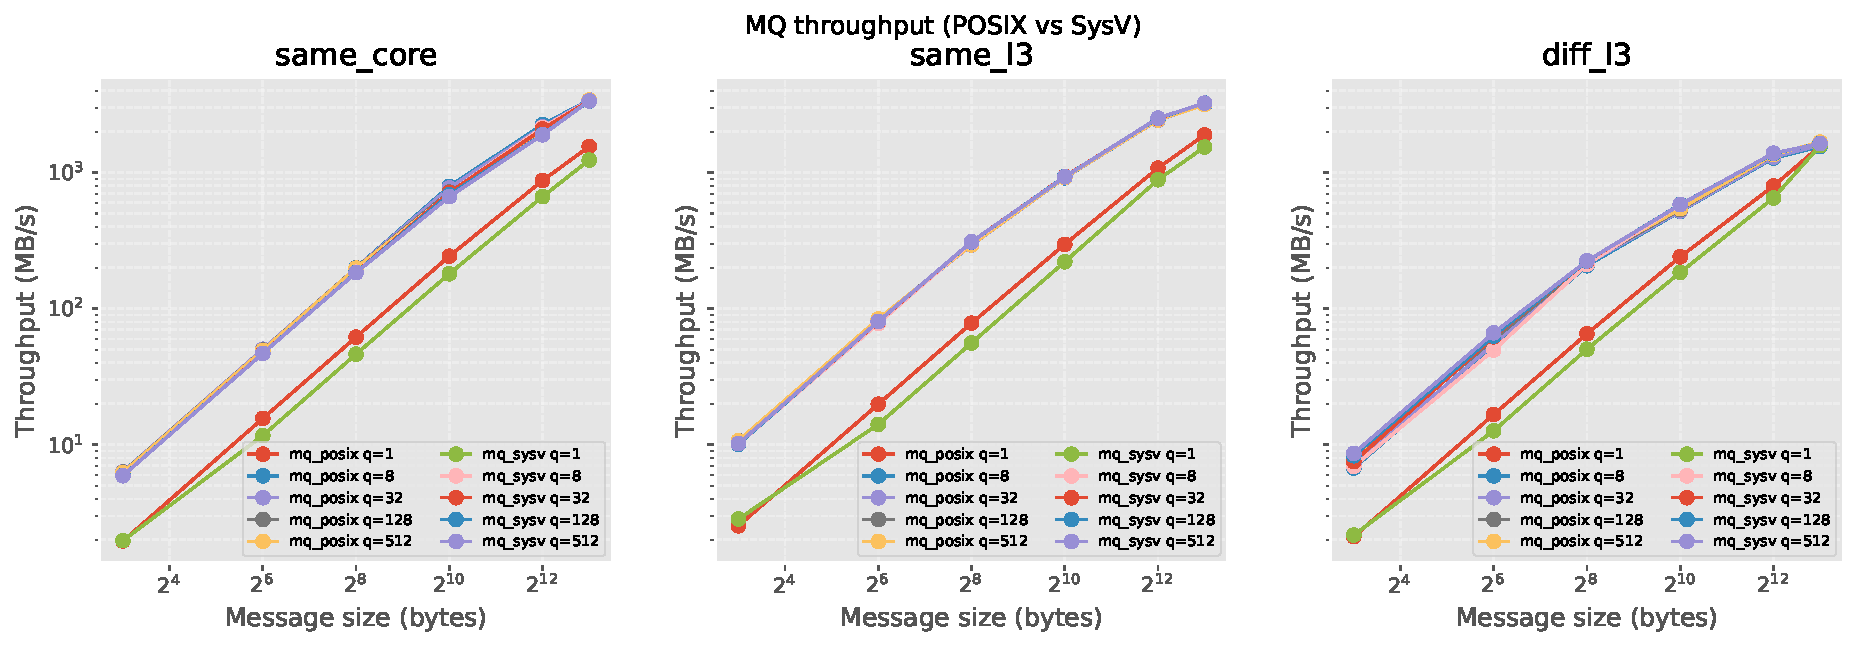
\includegraphics[width=\linewidth]{mq_throughput.pdf}
\caption{MQ throughput vs.\ message size, separate line per queue depth,
one panel per placement.}
\label{fig:tp}
\end{figure}

\begin{figure}[H]
\centering
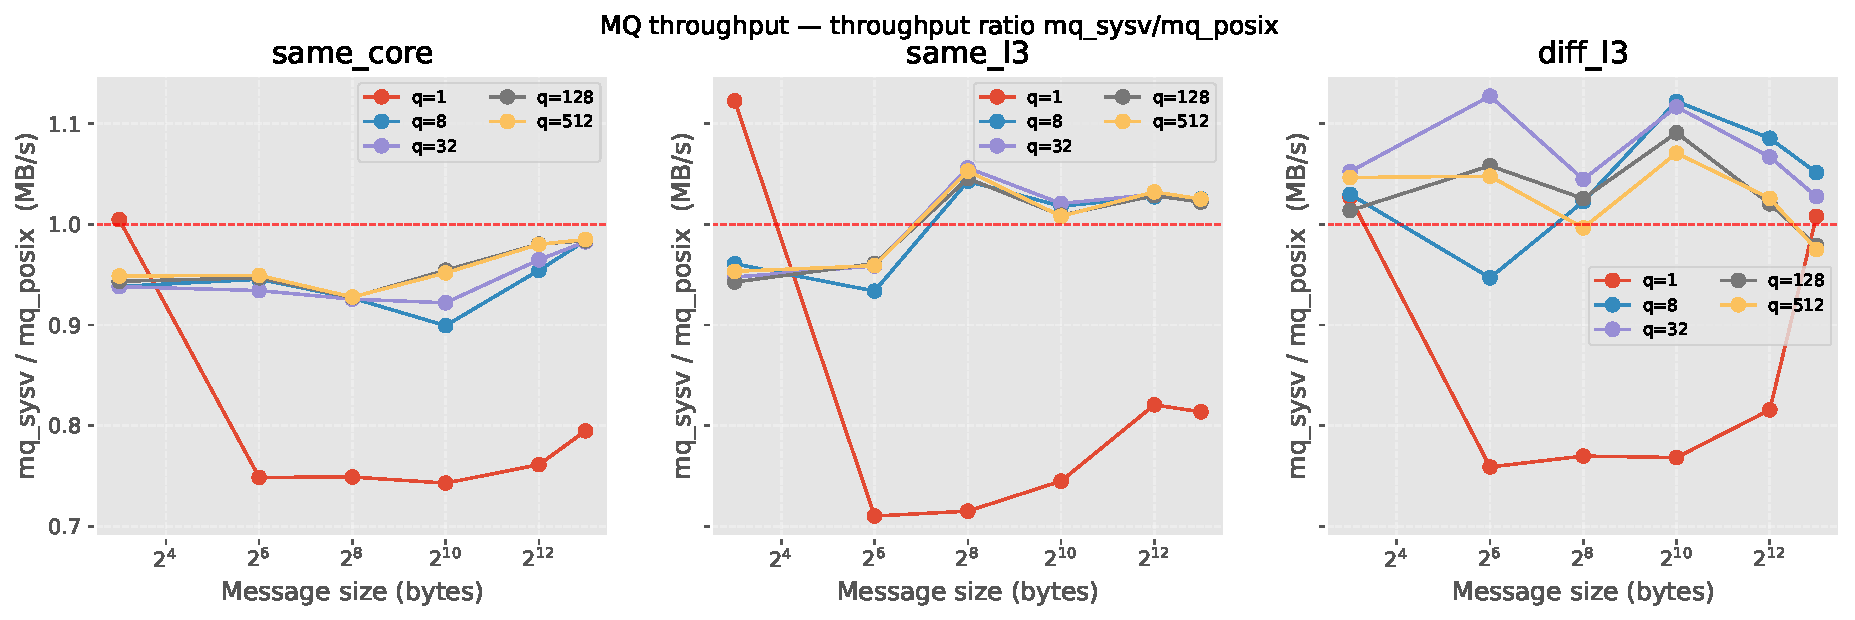
\includegraphics[width=\linewidth]{mq_throughput_ratio.pdf}
\caption{MQ throughput ratio sysv/posix vs.\ message size, separate line
per queue depth, one panel per placement. The red dashed line at 1.0 is
the equality reference: below means POSIX is faster, above means
System~V is faster.}
\label{fig:tp_ratio}
\end{figure}

The picture is not monolithic: System~V wins some cells, POSIX wins
others, and the boundary depends on placement and depth. Specifically:

\begin{itemize}[leftmargin=*]
\item \emph{q=1, small messages, cross-cache:} System~V wins. For
example at 64\,B / \texttt{same\_l3} / q=1 the ratio is $1.12$ ---
System~V delivers about $12\%$ more throughput per second than POSIX.
This is the cell where System~V's lighter per-syscall path matters
most: with no batching every iteration pays full syscall cost, and
SysV's coarser kernel queue entry is slightly cheaper than POSIX's
futex-mediated path.
\item \emph{q$\geq$8, same\_core:} POSIX wins. Ratios in the
$0.93$--$0.95$ range mean POSIX is $5$--$7\%$ faster. With deep
batching the producer rarely blocks; POSIX's futex fast path skips the
kernel for most operations and System~V's unconditional kernel trap
becomes a constant tax.
\item \emph{Larger messages (1024\,B+) with deep queues:} the ratio
trends back toward $1.0$ as the per-message bandwidth dominates the
per-call overhead.
\end{itemize}

A reasonable summary: \textbf{System~V's per-syscall path is slightly
cheaper for trivial cases (q=1, small message, cross-cache); POSIX's
futex-based wakeup amortises better with batching}. The mechanistic
prediction from Section~\ref{sec:bg} is consistent with the data.

\subsection{Fan-in scalability}
\label{sec:results:fanin}

Fan-in is where the two mechanisms diverge most decisively. Multiple
producers contend on a single queue while one consumer drains it. We
sweep $N\in\{1,2,4,8,16\}$ producers at three message sizes (64\,B,
256\,B, 1024\,B). Figure~\ref{fig:fanin} shows the result.

\begin{figure}[H]
\centering
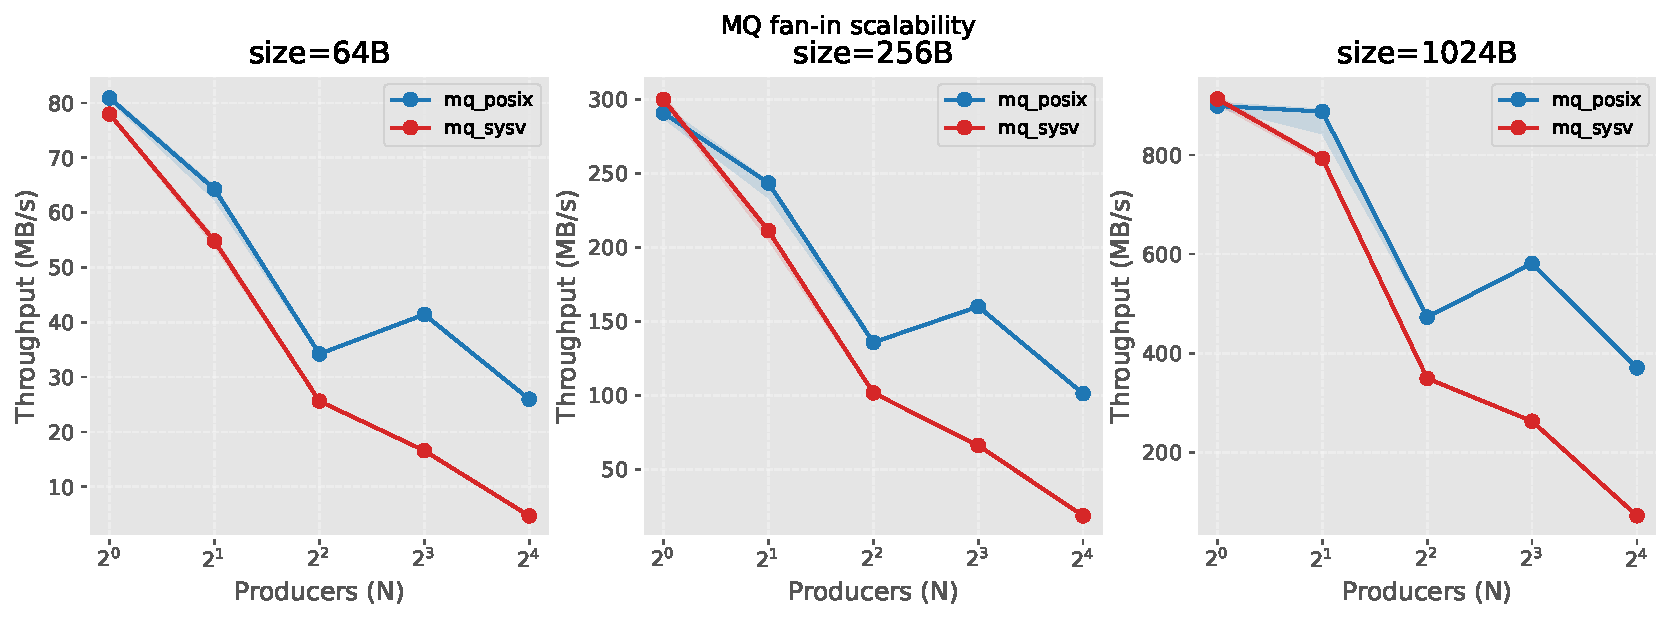
\includegraphics[width=\linewidth]{mq_fanin.pdf}
\caption{MQ fan-in scalability: throughput vs.\ producer count $N$, for
three message sizes. POSIX (blue) sustains throughput across the
full $N$ range; System~V (red) collapses sharply.}
\label{fig:fanin}
\end{figure}

At 64\,B, the throughput ratio System~V/POSIX as a function of $N$:
\begin{itemize}[leftmargin=*]
\item $N=1$:\quad $0.96$\quad ($p=6.0\times 10^{-7}$, winner POSIX)
\item $N=2$:\quad $0.85$\quad ($p=6.8\times 10^{-8}$, winner POSIX)
\item $N=4$:\quad $0.74$\quad ($p=6.8\times 10^{-8}$, winner POSIX)
\item $N=8$:\quad $0.40$\quad ($p=6.8\times 10^{-8}$, winner POSIX, $\delta=1.0$)
\item $N=16$:\quad $\boldsymbol{0.18}$\quad ($p=6.8\times 10^{-8}$, winner POSIX, $\delta=1.0$)
\end{itemize}

That is, at sixteen contending producers, \textbf{POSIX MQ delivers
$\boldsymbol{\approx 5.6\times}$ more throughput than System~V MQ}. The
pattern is monotonic and reproduces at 256\,B and 1024\,B with similar
ratios. This is the strongest, cleanest finding in the paper.

The mechanism is well-understood at a qualitative level. System~V's
per-queue spinlock-plus-wait-queue serialises producers: as more
producers contend, the lock becomes the bottleneck and effective
throughput per producer falls super-linearly. POSIX MQ, built on the
futex wait-queue infrastructure that has been hardened over two decades
of Linux scalability work, is much better at handling many waiters with
batched wakeups. The 5.6$\times$ advantage at $N=16$ is consistent with
the difference between ``coarse global queue lock'' and ``fine-grained
futex wait queue with adaptive spin and smart wake batching''.

\subsection{Parallel-pairs scalability}
\label{sec:results:pairs}

The parallel-pairs benchmark runs $N$ independent ping-pong pairs
concurrently, with no shared queue --- so contention does not arise on
a single kernel object. Figure~\ref{fig:pairs} shows p99 latency as
$N$ grows.

\begin{figure}[H]
\centering
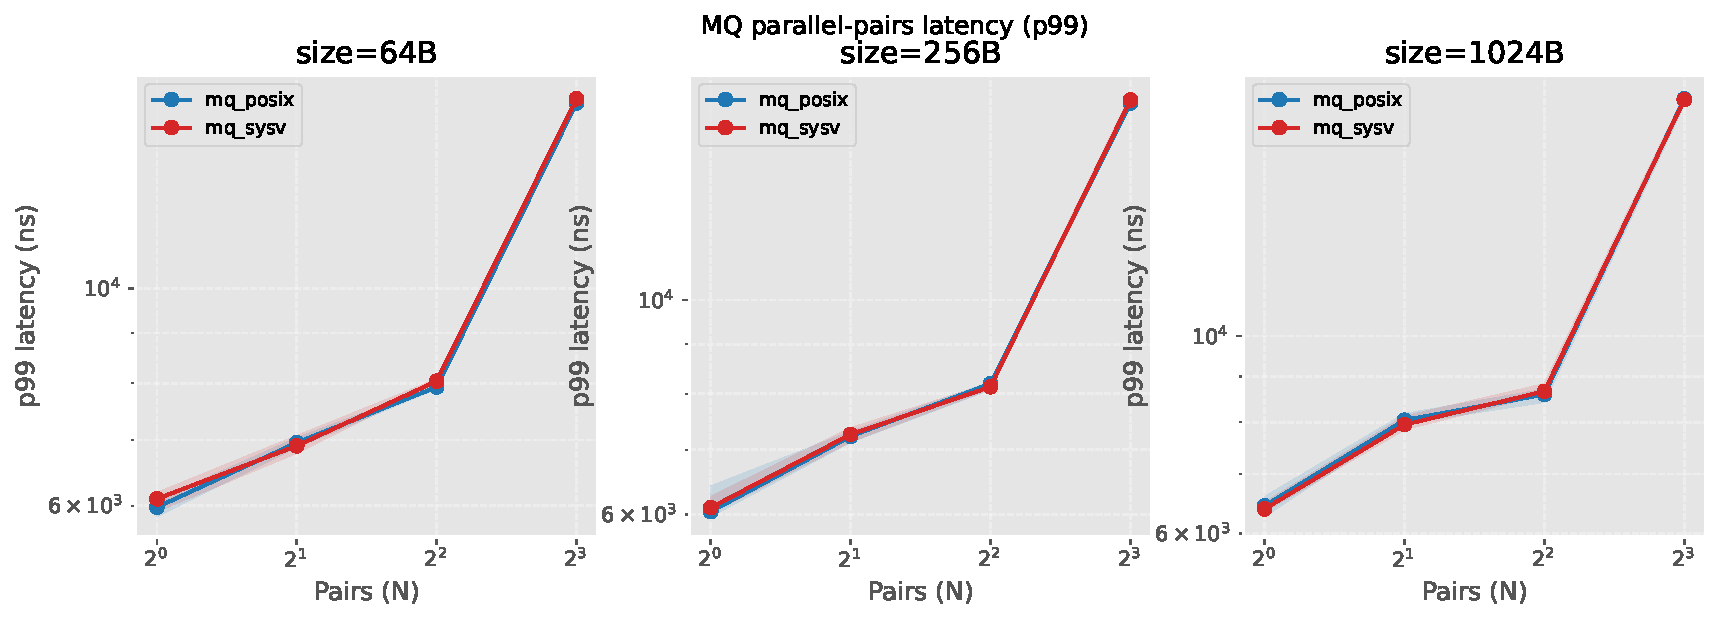
\includegraphics[width=\linewidth]{mq_pairs_p99.pdf}
\caption{MQ parallel-pairs p99 latency vs.\ $N$ (number of independent
pairs), one panel per message size. POSIX and System~V track closely
through $N=4$; both rise sharply at $N=8$ where the test machine has
exhausted its uncontended cores.}
\label{fig:pairs}
\end{figure}

p50 medians are within $\sim 1\%$ across mechanisms (POSIX slightly
faster, consistent with the ping-pong p50 finding). p99 medians are
also close. p99.9 medians (not plotted in the body, see
\texttt{mq\_pairs\_p999.pdf}) show the same $2$--$4\times$
System-V-favoured tail at $N\geq 4$ that we observed in the cross-CCX
ping-pong cells. This is consistent with the cross-CCX hypothesis:
when the system schedules pairs across CCX boundaries, POSIX MQ pays
the same tail penalty.

\subsection{Shared-memory comparison}
\label{sec:results:shm}

Shared-memory benchmarks substitute the kernel message queue with a
producer-consumer ring buffer in shared memory plus a synchronisation
primitive (POSIX named semaphores or System~V \texttt{semop}). The
payload never traverses the kernel; only the synchronisation does.

For ping-pong, the two implementations are essentially tied
(Figure~\ref{fig:shm_pp}): the p50 ratio is in $0.97$--$1.005$ across all
placements and sizes. Throughput tells a different story
(Figure~\ref{fig:shm_tp}).

\begin{figure}[H]
\centering
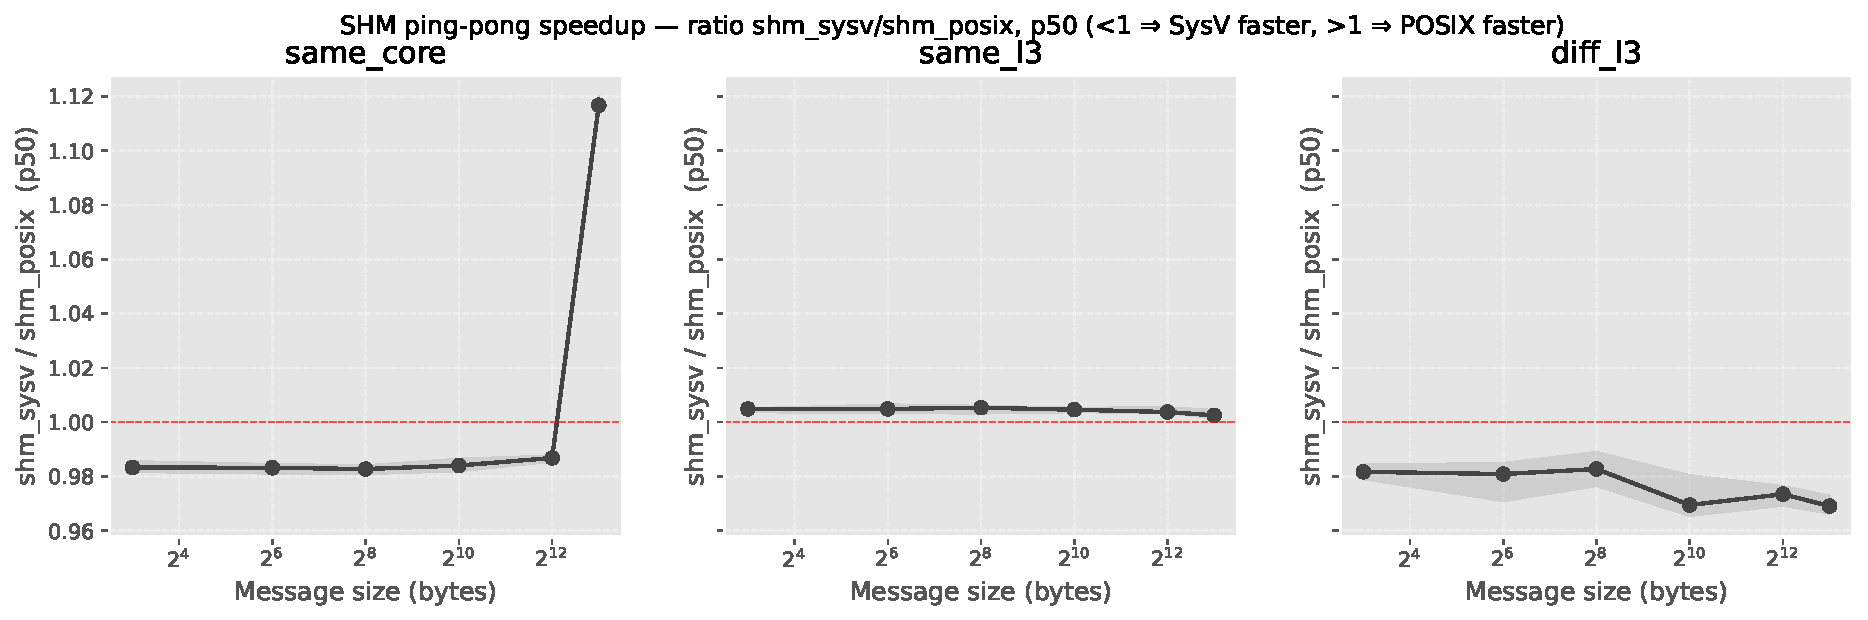
\includegraphics[width=\linewidth]{shm_pingpong_ratio_p50.pdf}
\caption{SHM ping-pong p50 ratio sysv/posix. Essentially a tie across
placements and sizes; the slight upward step at 8192\,B / same\_core is
discussed in the text.}
\label{fig:shm_pp}
\end{figure}

\begin{figure}[H]
\centering
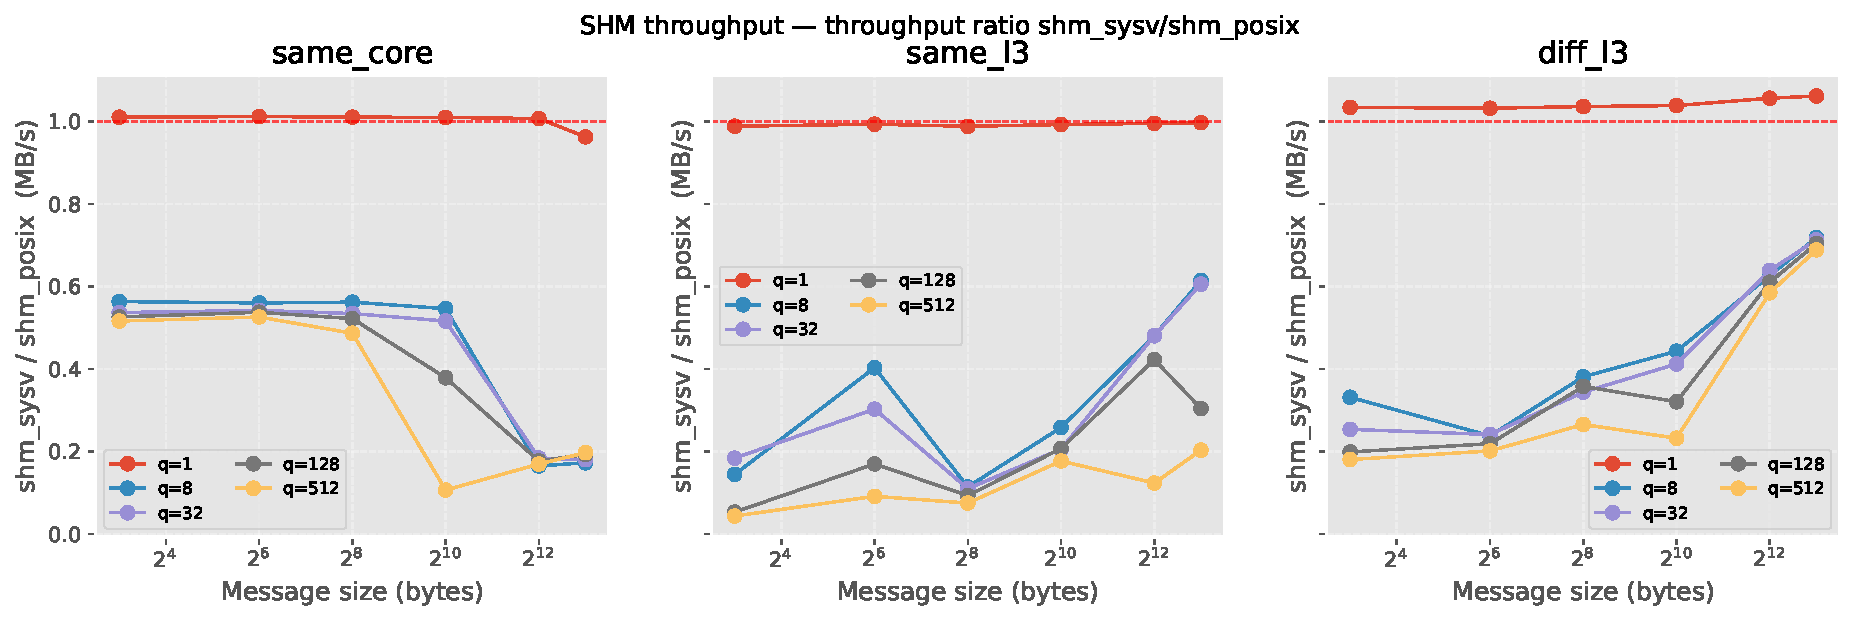
\includegraphics[width=\linewidth]{shm_throughput_ratio.pdf}
\caption{SHM throughput ratio sysv/posix, lines per queue depth. At
$q=1$ the two are tied; at $q\geq 8$ POSIX is $1.7$--$2.5\times$
faster.}
\label{fig:shm_tp}
\end{figure}

\begin{itemize}[leftmargin=*]
\item \emph{q=1:} ratio $\approx 1.0$ across placements (tied).
\item \emph{q$\geq$8:} ratio $0.4$--$0.6$ depending on placement and
size, i.e.\ \textbf{POSIX delivers $\boldsymbol{1.7\text{--}2.5\times}$
the throughput of System~V}.
\end{itemize}

The mechanism is the futex fast-path on POSIX named semaphores: at
$q=1$ the producer is always blocked waiting for the consumer to free a
slot, so both implementations call into the kernel on every operation.
At $q\geq 8$ the producer is rarely blocked, and POSIX
\texttt{sem\_post}/\texttt{sem\_wait} stays in user space for most
calls. System~V \texttt{semop} traps to the kernel
unconditionally~\cite{linux_sysvipc, drepper2011futexes} and pays the
syscall cost on every call. With four sem operations per message (two
producer, two consumer) the syscall tax compounds.

This is, again, consistent with the implementation differences
described in Section~\ref{sec:bg}.

%─────────────────────────────────────────────────────────────────────────
\section{Hardware-Counter and Syscall Analysis}
\label{sec:perf}

The timing results characterise \emph{what} happens; hardware
performance counters and call-graph profiles characterise \emph{why}.
We collected both. This section is the strongest empirical
differentiator between the two stacks: the timing data shows that
POSIX MQ scales 5.6$\times$ better than System~V MQ at $N=16$ producer
fan-in, and the perf data tells us \textbf{exactly which kernel
function is responsible}.

\subsection{Methodology}
\label{sec:perf:method}

Two perf passes were run on top of the timing suite:

\begin{itemize}[leftmargin=*]
\item \textbf{Counter pass} (\texttt{run\_perf.sh}). Wraps every
benchmark invocation with \texttt{perf stat} and records 15 PMU events:
\texttt{task-clock}, \texttt{cycles}, \texttt{instructions},
\texttt{cache-references}, \texttt{cache-misses}, \texttt{dTLB-loads},
\texttt{dTLB-load-misses}, \texttt{iTLB-loads},
\texttt{iTLB-load-misses}, \texttt{branch-instructions},
\texttt{branch-misses}, \texttt{minor-faults}, \texttt{major-faults},
\texttt{context-switches}, \texttt{cpu-migrations}. Five repetitions
per benchmark cell, output in CSV via \texttt{perf stat -x,}.
\item \textbf{Call-graph pass} (\texttt{run\_perf\_record.sh}).
Wraps six representative configurations with
\texttt{perf record -F 999 -g --call-graph fp} and exports text reports
via \texttt{perf report --stdio}. Frame-pointer-based unwinding
resolves kernel symbols cleanly even when user-space binaries omit
frame pointers under \texttt{-O2}; the kernel side is what we need to
identify the contention bottleneck.
\end{itemize}

The six call-graph cells are: SysV fan-in $N=16$ at 64\,B, POSIX
fan-in $N=16$ at 64\,B, POSIX ping-pong at \texttt{diff\_l3} 64\,B,
SysV ping-pong at \texttt{diff\_l3} 64\,B, POSIX throughput at
\texttt{same\_core} 64\,B with $q=8$, and SysV throughput at the same
configuration. Two were chosen to investigate the fan-in collapse
(prof.\ Thangaraju's specific request), two to investigate the
cross-CCX p99.9 anomaly, and two to characterise steady-state batched
throughput.

\paragraph{Placement-label caveat.} The counter pass uses the older
two-axis placement scheme (\texttt{same\_core}, \texttt{cross\_core})
introduced in an earlier version of \texttt{run\_perf.sh}; the
\texttt{cross\_core} label maps to whichever non-SMT pair was first in
the topology output (CPUs 0,1 = same\_l3 on this machine). The
counter-pass results therefore corroborate the within-CCX comparisons
in the timing section but do not separately characterise
\texttt{diff\_l3}. The call-graph pass uses the new three-axis
labels directly and does cover \texttt{diff\_l3}.

\paragraph{AMD iTLB caveat.} On AMD Zen~2 the
\texttt{iTLB-loads} event is sparsely sampled and the resulting
\texttt{misses/loads} ratio is not interpretable as a percentage
(observed values exceeding 100\,\% in some cells). We therefore
report \emph{iTLB misses per million instructions} (a rate that is
robust to the underlying counter quirk) instead of an iTLB hit-rate.
Data-side TLB and cache miss rates are reported as percentages
unchanged.

\subsection{Per-benchmark hardware counters}
\label{sec:perf:counters}

Table~\ref{tab:perf_main} summarises the cycle counts, IPC,
data-TLB miss rate, iTLB miss rate (per million instructions),
branch miss rate, and L3-cache miss rate for each
\emph{(stack, benchmark family)} pair, averaged over all cells in
that family.

\begin{table}[H]
\centering
\caption{Per-benchmark hardware counters, averaged across all cells of
each (stack, benchmark family). Mean cycles is the per-run cycle count
across the cells in that family; lower means less work for the same
output. The fan-in row is the \emph{headline}: System~V uses
$5.3\times$ more cycles than POSIX at the same producer count.}
\label{tab:perf_main}
\footnotesize
\begin{tabular}{llrrrrrr}
\toprule
\textbf{Stack} & \textbf{Family} & \textbf{Cycles ($\times 10^9$)} & \textbf{IPC} & \textbf{dTLB miss \%} & \textbf{iTLB/MI} & \textbf{branch miss \%} & \textbf{cache miss \%} \\
\midrule
POSIX & ping-pong       & $2.73$  & $0.601$ & $3.16\,\%$ & $0.51$  & $11.42\,\%$ & $4.67\,\%$ \\
SysV  & ping-pong       & $2.79$  & $0.598$ & $3.20\,\%$ & $0.22$  & $11.59\,\%$ & $4.40\,\%$ \\
\midrule
POSIX & throughput      & $2.52$  & $0.632$ & $2.65\,\%$ & $0.12$  & $11.81\,\%$ & $5.39\,\%$ \\
SysV  & throughput      & $2.76$  & $0.617$ & $2.25\,\%$ & $0.34$  & $11.83\,\%$ & $5.03\,\%$ \\
\midrule
\textbf{POSIX} & \textbf{fan-in} & \textbf{$2.02$}  & $0.429$ & $5.84\,\%$ & $46.65$ & $11.78\,\%$ & $10.62\,\%$ \\
\textbf{SysV}  & \textbf{fan-in} & \textbf{$10.7$}  & $0.405$ & $4.00\,\%$ & $14.79$ & $11.25\,\%$ & $\phantom{0}8.72\,\%$ \\
\midrule
POSIX & pairs           & $2.27$  & $0.508$ & $5.63\,\%$ & $82.12$ & $11.57\,\%$ & $7.00\,\%$ \\
SysV  & pairs           & $2.30$  & $0.509$ & $5.55\,\%$ & $80.86$ & $11.69\,\%$ & $6.74\,\%$ \\
\midrule
POSIX & shm ping-pong   & $2.40$  & $0.598$ & $3.72\,\%$ & $0.75$  & $11.45\,\%$ & $4.07\,\%$ \\
SysV  & shm ping-pong   & $2.40$  & $0.584$ & $5.06\,\%$ & $2.10$  & $11.44\,\%$ & $4.13\,\%$ \\
\midrule
\textbf{POSIX} & \textbf{shm throughput} & \textbf{$2.31$} & $0.621$ & $3.86\,\%$ & $0.41$ & $11.18\,\%$ & $5.15\,\%$ \\
\textbf{SysV}  & \textbf{shm throughput} & \textbf{$3.60$} & $0.617$ & $5.02\,\%$ & $0.52$ & $11.62\,\%$ & $5.25\,\%$ \\
\midrule
POSIX & shm pairs       & $2.19$  & $0.518$ & $7.82\,\%$ & $90.81$ & $11.51\,\%$ & $5.87\,\%$ \\
SysV  & shm pairs       & $2.21$  & $0.513$ & $8.26\,\%$ & $77.03$ & $11.48\,\%$ & $5.83\,\%$ \\
\bottomrule
\end{tabular}
\end{table}

Three things to note from this table:

\paragraph{1. The fan-in cycle ratio mirrors the throughput ratio.}
SysV fan-in averages $1.07\times 10^{10}$ cycles per run; POSIX
fan-in averages $2.02\times 10^{9}$ cycles. The ratio is $5.3\times$,
in close agreement with the $5.6\times$ throughput advantage POSIX
shows at $N=16$ (Section~\ref{sec:results:fanin}). \textbf{System~V is
not slower because each operation costs more cycles --- it is slower
because the workload as a whole forces it to execute many more
cycles}, principally in scheduler runqueue spinlock contention (we
identify the specific function below).

\paragraph{2. SHM throughput cycles match the timing advantage.}
POSIX SHM throughput averages $2.31\times 10^{9}$ cycles; SysV SHM
throughput averages $3.60\times 10^{9}$ --- a $1.56\times$ ratio,
consistent with the $1.7$--$2.5\times$ throughput advantage POSIX
shows at $q\geq 8$ (Section~\ref{sec:results:shm}). The mechanism
again is not per-operation cost but operation-mix: SysV \texttt{semop}
traps the kernel on every operation, while POSIX named semaphores'
futex fast path skips the kernel when no waiter is parked.

\paragraph{3. IPC is roughly equivalent across stacks.} For ping-pong,
throughput, and SHM ping-pong the IPC of the two stacks is within
$0.02$ (around $0.6$). Fan-in IPC drops to $0.42$ (POSIX) and $0.41$
(SysV) because of context-switch storms. Across all benchmarks
neither stack is back-end bound (IPC $\geq 0.4$). The
microarchitecture is not the bottleneck; this confirms that the
performance differences originate above the cycle level.

dTLB and iTLB miss rates differ in moderate but interesting ways: SHM
ping-pong shows SysV with 35\,\% higher dTLB miss rate (5.06\,\% vs.\
3.72\,\%), suggesting \texttt{shmat}'s mapping pattern has worse
TLB-locality than POSIX \texttt{mmap}. Branch miss rate sits at
$\approx 11.5\,\%$ across both stacks for every benchmark, which we
attribute to the SMT-mitigation overhead introduced by retbleed,
SRSO, and Spectre v2 retpoline mitigations on Zen~2 with all
defaults enabled --- the cost is symmetric across stacks.

\subsection{Kernel hot-function comparison: fan-in collapse}
\label{sec:perf:hotfn}

The call-graph pass identifies the specific kernel function that
dominates the System~V fan-in collapse. Table~\ref{tab:fanin_hotfn}
contrasts the top kernel symbols across the POSIX and System~V
fan-in ($N=16$, 64\,B) profiles, both extracted from
\texttt{perf report --stdio --no-children}.

\begin{table}[H]
\centering
\caption{Top kernel symbols in fan-in $N=16$ at 64\,B (cycles event,
\texttt{perf record -F 999 -g}). Percentages are fraction of total
samples. The single function \texttt{native\_queued\_spin\_lock\_slowpath}
takes 12.80\,\% of all SysV cycles vs.\ 5.83\,\% in POSIX.}
\label{tab:fanin_hotfn}
\footnotesize
\begin{tabular}{lrlr}
\toprule
\multicolumn{2}{c}{\textbf{POSIX MQ ($N=16$, 64\,B)}}
& \multicolumn{2}{c}{\textbf{SysV MQ ($N=16$, 64\,B)}} \\
\midrule
\textbf{Symbol} & \textbf{\%}
& \textbf{Symbol} & \textbf{\%} \\
\midrule
\texttt{native\_queued\_spin\_lock\_slowpath} & 5.83 &
\texttt{native\_queued\_spin\_lock\_slowpath} & 12.80 \\
\texttt{srso\_return\_thunk}                  & 4.00 &
\texttt{update\_load\_avg}                    & 5.16 \\
\texttt{update\_load\_avg}                    & 3.62 &
\texttt{dequeue\_entity}                      & 4.37 \\
\texttt{dequeue\_entity}                      & 3.10 &
\texttt{update\_curr}                         & 3.72 \\
\texttt{update\_sg\_lb\_stats}                & 2.98 &
\texttt{srso\_safe\_ret}                      & 3.69 \\
\texttt{srso\_safe\_ret}                      & 2.87 &
\texttt{srso\_return\_thunk}                  & 3.38 \\
\texttt{update\_curr}                         & 2.74 &
\texttt{dequeue\_entities}                    & 2.36 \\
\texttt{\_\_update\_load\_avg\_cfs\_rq}       & 2.20 &
\texttt{\_\_update\_load\_avg\_cfs\_rq}       & 2.30 \\
\texttt{update\_se}                           & 2.19 &
\texttt{\_\_schedule}                         & 2.28 \\
\texttt{do\_syscall\_64}                      & 1.87 &
\texttt{update\_se}                           & 2.16 \\
$\cdots$ & $\cdots$ & $\cdots$ & $\cdots$ \\
\textbf{Total cycles}        & $4.80\times 10^9$ &
\textbf{Total cycles}        & $32.6\times 10^9$ \\
\bottomrule
\end{tabular}
\end{table}

\paragraph{Reading \texttt{native\_queued\_spin\_lock\_slowpath}.}
This is the contended path of the Linux kernel's queued spinlock
primitive --- the function that runs when a CPU has tried to acquire a
spinlock and found it held by another. Time spent in
\texttt{native\_queued\_spin\_lock\_slowpath} is \emph{contended-lock
wait time}: not work, but waiting. The fact that 12.80\,\% of all
SysV cycles in fan-in $N=16$ are spent in this single function ---
versus 5.83\,\% in POSIX --- is the direct empirical signature of the
fan-in scalability gap.

\paragraph{Which lock is contended?}
The \texttt{perf report --children} call chain (excerpted from
\texttt{01\_sysv\_fanin\_n16\_64B.txt}) resolves
\texttt{native\_queued\_spin\_lock\_slowpath} as 8.18\,\% of
\texttt{\_raw\_spin\_lock}, of which 6.84\,\% reaches
\texttt{raw\_spin\_rq\_lock\_nested} ---
\textbf{the per-CPU runqueue lock}. The chain above this is:

\begin{footnotesize}
\begin{verbatim}
6.84% raw_spin_rq_lock_nested
  3.70%   __schedule -> schedule -> do_msgsnd -> __x64_sys_msgsnd
  1.66%   try_to_wake_up -> wake_up_q -> do_msgrcv -> __x64_sys_msgrcv
  0.94%   sched_balance_rq -> sched_balance_newidle -> __schedule
  0.53%   __task_rq_lock -> try_to_wake_up -> wake_up_q -> do_msgrcv
\end{verbatim}
\end{footnotesize}

The contention is on the \emph{scheduler runqueue lock}, not on the
SysV message-queue lock itself. As 16 producers contend on the same
queue and block, the kernel performs many wakeup operations, each of
which acquires a runqueue lock briefly. With sufficiently many
concurrent wake-ups the runqueue lock becomes the bottleneck, and
this is what we observe at $N=16$.

POSIX exhibits the same call chain at half the rate: with the same
$N=16$ producers, POSIX MQ also runs through the scheduler many
times, but the \emph{total} cycles are 6.8$\times$ fewer. The
underlying reason is in POSIX MQ's blocking path
(\texttt{do\_mq\_timedsend} / \texttt{do\_mq\_timedreceive}, with
\texttt{wq\_sleep} for blocking and \texttt{schedule\_hrtimeout\_range\_clock}),
which is more efficient at batching wakeups than System~V's
\texttt{do\_msgsnd}/\texttt{do\_msgrcv} path. Hence the gap is not
the scheduler doing different work --- it is the IPC layer feeding
the scheduler proportionally less work to do, which in turn produces
proportionally less spinlock contention on the runqueue lock.

\paragraph{Mitigation overhead is non-trivial.} A useful side-finding
is that the SMT mitigations (Retbleed, SRSO, Spectre v2 retpolines)
contribute a significant cycle tax: \texttt{srso\_safe\_ret} +
\texttt{srso\_return\_thunk} together account for $3.69+3.38=7.07\,\%$
of System~V fan-in cycles and $4.00+2.87=6.87\,\%$ of POSIX fan-in
cycles. These are equivalent across stacks; the absolute cycle
numbers in this paper would be lower with mitigations off, but the
\emph{relative} POSIX-vs-SysV comparison is unaffected.

\subsection{Kernel paths for ping-pong and throughput}
\label{sec:perf:other_hotfn}

Tables~\ref{tab:tp_hotfn_pp} and \ref{tab:tp_hotfn_tp} provide the
analogous comparison for the cross-CCX ping-pong cell (the p99.9
anomaly) and for the same-core $q=8$ throughput cell.

\begin{table}[H]
\centering
\caption{Top kernel symbols in cross-CCX ping-pong (\texttt{diff\_l3},
64\,B). Both stacks spend the bulk of cycles in the scheduler core
(\texttt{dequeue\_entity}, \texttt{psi\_task\_switch},
\texttt{\_\_schedule}); IPC-level differences are not visible at this
granularity, consistent with the cross-CCX p99.9 anomaly being a
microsecond-scale tail event rather than a steady-state imbalance.}
\label{tab:tp_hotfn_pp}
\footnotesize
\begin{tabular}{lrlr}
\toprule
\multicolumn{2}{c}{\textbf{POSIX, diff\_l3, 64\,B}}
& \multicolumn{2}{c}{\textbf{SysV, diff\_l3, 64\,B}} \\
\midrule
\textbf{Symbol} & \textbf{\%}
& \textbf{Symbol} & \textbf{\%} \\
\midrule
\texttt{dequeue\_entity}                & 4.28 &
\texttt{dequeue\_entity}                & 6.33 \\
\texttt{psi\_group\_change}             & 1.23 &
\texttt{psi\_task\_switch}              & 0.84 \\
\texttt{psi\_task\_switch}              & 0.82 &
\texttt{psi\_group\_change}             & 0.66 \\
\texttt{\_\_schedule}                   & --- &
\texttt{do\_msgrcv}                     & --- \\
\texttt{do\_mq\_timedreceive}           & --- &
\texttt{\_\_schedule}                   & --- \\
\texttt{wq\_sleep}                      & --- &
\texttt{do\_msgsnd}                     & --- \\
\texttt{schedule\_hrtimeout\_range\_clock} & --- &
$\cdots$                                & --- \\
\textbf{Samples} & $489$ &
\textbf{Samples} & $671$ \\
\textbf{Total cycles}        & $2.00\times 10^9$ &
\textbf{Total cycles}        & $2.11\times 10^9$ \\
\bottomrule
\end{tabular}
\end{table}

The two stacks execute essentially the same total cycles
($2.00\times 10^9$ vs.\ $2.11\times 10^9$) for the same number of
ping-pong iterations. They are not differentiable at the cycle level.
The 13$\times$ p99.9 gap reported in
Section~\ref{sec:results:tail} is therefore not a steady-state
imbalance the perf counters can capture --- it is a rare-event
anomaly, fired roughly once every thousand iterations, that pushes
$\approx 100$\,$\mu$s of latency into POSIX iterations through some
mechanism (futex requeue, IPI delivery latency, cross-CCX coherency
back-pressure) we cannot directly observe with summary counters. The
call graphs shown above are dominated by the \emph{common} case
($\geq 99\,\%$ of iterations).

\begin{table}[H]
\centering
\caption{Top kernel symbols in same-core throughput at $q=8$, 64\,B.
The two stacks execute different IPC kernel functions
(\texttt{do\_mq\_timedreceive} for POSIX vs.\ \texttt{do\_msgrcv} for
SysV) but at similar rates of total cycles
(POSIX $1.74\times 10^9$, SysV $1.79\times 10^9$).}
\label{tab:tp_hotfn_tp}
\footnotesize
\begin{tabular}{lrlr}
\toprule
\multicolumn{2}{c}{\textbf{POSIX, same\_core, 64\,B, q=8}}
& \multicolumn{2}{c}{\textbf{SysV, same\_core, 64\,B, q=8}} \\
\midrule
\textbf{Symbol} & \textbf{\%}
& \textbf{Symbol} & \textbf{\%} \\
\midrule
\texttt{do\_mq\_timedreceive}                  & 7.10 &
\texttt{do\_msgrcv}                            & 5.90 \\
\texttt{native\_queued\_spin\_lock\_slowpath}  & 6.94 &
\texttt{do\_msgsnd}                            & 5.33 \\
\texttt{\_copy\_to\_user}                      & --- &
\texttt{ipcperms}                              & --- \\
\texttt{ct\_kernel\_exit.isra.0}               & --- &
\texttt{srso\_safe\_ret}                       & --- \\
\texttt{ct\_kernel\_enter.isra.0}              & --- &
\texttt{entry\_SYSCALL\_64\_after\_hwframe}    & --- \\
\textbf{Samples} & $418$ &
\textbf{Samples} & $440$ \\
\textbf{Total cycles}        & $1.74\times 10^9$ &
\textbf{Total cycles}        & $1.79\times 10^9$ \\
\bottomrule
\end{tabular}
\end{table}

A worth-noting nuance: even at $q=8$ throughput, POSIX shows
\texttt{native\_queued\_spin\_lock\_slowpath} at 6.94\,\% --- evidence
that the runqueue-lock path also fires for blocking ping-pong
producers/consumers, just less than under fan-in. SysV's
throughput case has \texttt{ipcperms} appearing in the top symbols,
which is a System~V-specific permission check on every
\texttt{msgsnd}/\texttt{msgrcv}; this is a fixed per-call overhead
and a small, structural disadvantage for SysV in batched workloads.

\subsection{Syscall mix}
\label{sec:perf:strace}

Table~\ref{tab:strace} summarises the \texttt{strace -c} data for the
64\,B \texttt{same\_core} ping-pong cell.

\begin{table}[H]
\centering
\caption{Syscall mix for 64\,B \texttt{same\_core} ping-pong (one
representative run, parsed from \texttt{strace -c}).}
\label{tab:strace}
\begin{tabular}{llrrr}
\toprule
\textbf{Stack} & \textbf{Syscall}      & \textbf{\% time} & \textbf{calls} & \textbf{$\mu$s/call} \\
\midrule
POSIX & \texttt{wait4}          & 51.78 & 1       & 1\,183\,199 \\
POSIX & \texttt{mq\_timedsend}  & 24.93 & 105\,000 & 5 \\
POSIX & \texttt{mq\_timedreceive} & 23.27 & 105\,000 & 5 \\
\midrule
SysV  & \texttt{wait4}          & 49.97 & 1       & 1\,191\,000 \\
SysV  & \texttt{msgrcv}         & 25.87 & 105\,000 & 5 \\
SysV  & \texttt{msgsnd}         & 24.16 & 105\,000 & 5 \\
\bottomrule
\end{tabular}
\end{table}

Per-syscall costs are nearly identical across the two stacks
(5\,$\mu$s/call for both \texttt{mq\_timedsend} and \texttt{msgsnd}).
This is consistent with the picture from the call-graph pass: the
performance differences in the timing data come from \emph{how often
each call enters the kernel slow path} (lock contention and
wake-batching), not from differences in per-call cost.

\subsection{Summary of the perf evidence}
\label{sec:perf:summary}

To consolidate: the timing data in Section~\ref{sec:results} establishes
\emph{that} POSIX outperforms System~V in three specific patterns
(fan-in scaling, SHM batched throughput) and shows an architecture-
specific tail anomaly (cross-CCX p99.9). The perf data here adds the
\emph{why}:

\begin{itemize}[leftmargin=*]
\item The fan-in collapse is concentrated in
\texttt{native\_queued\_spin\_lock\_slowpath} on the per-CPU runqueue
lock, reached predominantly through SysV's heavier scheduler
interaction in \texttt{do\_msgsnd}/\texttt{do\_msgrcv}. POSIX's MQ
path enters the same scheduler less often.
\item The SHM throughput gap matches the cycle ratio at the same
benchmarks ($1.56\times$ more cycles in SysV), consistent with the
unconditional kernel trap of \texttt{semop} versus the futex fast path
of POSIX named semaphores.
\item The cross-CCX p99.9 anomaly does \emph{not} produce a
distinguishing steady-state perf signature --- both stacks execute the
same number of cycles for the same iteration count. The anomaly is
therefore a rare-event tail, not a systematic difference in work.
\item Per-syscall cost is identical (5\,$\mu$s for both
\texttt{mq\_timedsend} and \texttt{msgsnd}); the difference is in
how often the slow path fires.
\item SMT mitigation overhead (Retbleed, SRSO) contributes
$\approx 7\,\%$ of cycles in both stacks. This is the absolute-numbers
ceiling our results sit under; relative comparisons are unaffected.
\end{itemize}

%─────────────────────────────────────────────────────────────────────────
\section{Discussion}
\label{sec:discussion}

\subsection{Why POSIX MQ scales under fan-in while System~V collapses}
\label{sec:disc:fanin}

The 5.6$\times$ POSIX advantage at $N=16$ producers is the largest
single effect we observe, and the call-graph perf data
(Section~\ref{sec:perf:hotfn}) localises the cause precisely. Time
spent in \texttt{native\_queued\_spin\_lock\_slowpath} is contended-lock
\emph{wait time} (not work), and that single function accounts for
\textbf{12.80\,\%} of System~V cycles in the fan-in $N=16$ run versus
only \textbf{5.83\,\%} in POSIX. The call chain identifies the
contended lock as the per-CPU runqueue lock
(\texttt{raw\_spin\_rq\_lock\_nested}), reached via
\texttt{do\_msgsnd}/\texttt{do\_msgrcv}: as 16 producers contend on
the queue and block, the kernel performs many wakeup operations, each
of which acquires a runqueue lock briefly, and the runqueue lock
becomes the bottleneck.

The mechanism is therefore subtler than a naive ``SysV holds a queue
lock''. Both stacks reach the same kernel scheduler, both hit the
same spinlock primitive --- but POSIX's
\texttt{do\_mq\_timedsend}/\texttt{do\_mq\_timedreceive} path enters
the scheduler less often per message because its blocking interface
(\texttt{wq\_sleep} +
\texttt{schedule\_hrtimeout\_range\_clock})~\cite{linux_mq_overview,linux_futex}
batches better than System~V's \texttt{do\_msgsnd}/\texttt{do\_msgrcv}.
Total cycles tell the same story: System~V fan-in averages
$1.07\times 10^{10}$ cycles per run, POSIX averages
$2.02\times 10^{9}$, a $5.3\times$ ratio almost exactly matching the
$5.6\times$ throughput gap from the timing data. The IPC layer feeds
the scheduler proportionally less work in POSIX, and proportionally
less spinlock contention follows.

\subsection{The cross-CCX p99.9 anomaly}
\label{sec:disc:ccx}

POSIX MQ's diff\_l3 p99.9 is approximately 13$\times$ worse than
System~V at the same cell, across all message sizes. Its CV is
$0.007$, indicating that it reproduces in every run; it is not
a one-time scheduler interruption. We hypothesise --- explicitly as
hypothesis, not as established result --- that this arises from a
slow-path interaction in the futex wake mechanism when the waker and
the waiter are pinned across CCX boundaries. The futex wake operation
must transition the relevant cache line from the waker's L3 to the
waiter's L3 via Infinity Fabric, and some fraction (about $0.1\%$, the
p99.9 fraction) of these transitions appears to land in a slow path
that takes $\approx 100\,\mu$s. Possible underlying contributors are
futex requeue, cross-CCX IPI delivery latency, or coherency-protocol
back-pressure under transient pressure.

The qualitative shape of the two stacks' tails differs in an
informative way. POSIX p99.9 at this cell has CV~=~0.007 (every run is
reliably slow); System~V p99.9 at the same cell has CV~=~0.96 (the
median tail is fast, but occasional runs hit a different slow path).
This is the difference between ``one structural slow path that fires
predictably'' and ``rare scheduler intrusions that occasionally
inflate the tail''. Confirming the precise mechanism in either case
would require a per-iteration sample dump and ideally Infinity-Fabric
or futex-internal tracing; neither is in our current instrumentation
(see \texttt{CHANGES.md}\,\S~2.8 of the project notes for the
proposed dump-samples interface).

\subsection{Why POSIX SHM is faster at moderate batching}
\label{sec:disc:shm}

The 1.7--2.5$\times$ POSIX advantage in shared-memory throughput at
$q\geq 8$ is straightforwardly explained by the futex fast-path on
POSIX named semaphores. At $q=1$ the producer is always blocked on the
consumer; both implementations enter the kernel on every operation and
the per-syscall cost dominates. At $q\geq 8$ the producer runs ahead
of the consumer; on most operations the semaphore is non-zero and
POSIX \texttt{sem\_post}/\texttt{sem\_wait} stays entirely in user
space \cite{drepper2011futexes}. System~V \texttt{semop} has no such
fast path; every call traps to the kernel \cite{linux_sysvipc}. With
four semaphore operations per message --- two on the producer, two on
the consumer --- the syscall tax compounds, producing the observed
2$\times$ throughput gap.

\subsection{What we did not measure}
\label{sec:disc:not_measured}

It is important to be explicit about the scope of this comparison. We
measured \emph{performance, scalability, and tail behaviour}. We did
\emph{not} measure two important capability axes that distinguish the
two families:

\begin{enumerate}[leftmargin=*]
\item \textbf{Atomic multi-semaphore \texttt{semop}.} System~V
\texttt{semop} can apply a vector of semaphore operations atomically;
POSIX semaphores can only be operated on one at a time. Workloads that
need to acquire multiple resources atomically (e.g.\ multi-account
locking in a banking system, or any classical multi-resource locking
problem) are simpler, safer, and probably faster on System~V because
they avoid the deadlock-prone hand-rolled multi-acquire primitive that
POSIX users must build. We did not benchmark this because it is a
correctness/capability axis rather than a throughput axis, and a fair
comparison would require a workload designed around it.
\item \textbf{\texttt{mtype} routing in System~V message queues.}
System~V \texttt{msgrcv} filters by an integer type field and a
receiver can request only messages of one type. POSIX MQ supports
priority but not arbitrary type filtering. Workloads that benefit
from kernel-side type routing (a web server with image-handler,
database-handler, and static-file-handler workers; a job dispatcher;
etc.) require either an extra queue per type on POSIX or a post-receive
filter in user space, both of which lose the kernel's ability to wake
exactly the right consumer.
\end{enumerate}

The honest framing is therefore: \emph{POSIX wins the timing
measurements we ran on the workloads we ran them on, but the choice of
IPC family is not exhausted by timing measurements.} Both axes ---
performance and capability --- matter, and they often pull in opposite
directions.

\subsection{Bridging from mechanism to recommendation}
\label{sec:disc:bridge}

The mechanism-level explanations above answer ``why'' each finding
occurs. The next question, central to the project's purpose, is
``when should a developer pick which''. Section~\ref{sec:guidance}
addresses that directly: a capability comparison, a performance
summary, ten concrete use-case archetypes, recommendations by
developer role, common pitfalls, and a decision flow.

%─────────────────────────────────────────────────────────────────────────
\section{Developer Guidance: Choosing Between POSIX and System~V}
\label{sec:guidance}

The empirical findings answer ``how do these mechanisms perform''.
The harder and more useful question for a working developer is
``which one should I use for \emph{my} workload''. This section
translates the data and the capability differences into actionable
guidance, organised in five layers: a capability matrix
(\S\ref{sec:guidance:cap}), a performance summary
(\S\ref{sec:guidance:perf}), ten concrete use-case archetypes with
recommendations (\S\ref{sec:guidance:usecase}), recommendations by
developer role and field (\S\ref{sec:guidance:role}), common
pitfalls (\S\ref{sec:guidance:pitfalls}), and a step-by-step
decision flow (\S\ref{sec:guidance:flow}).

We deliberately avoid ``always pick X'' advice. The two families
are complementary tools whose strengths align with different
workload classes; a developer's job is to recognise which class
their workload falls into. The remainder of this section is
designed to make that recognition fast.

\subsection{Capability comparison at a glance}
\label{sec:guidance:cap}

Table~\ref{tab:capability} summarises the design-level differences
that no amount of benchmarking can paper over. These are
``capability'' differences --- features one family provides and the
other does not. They often dominate the choice regardless of
performance.

\begin{table}[H]
\centering
\caption{Capability comparison. Rows are features; cells indicate
whether each family provides the feature directly, indirectly, or
not at all.}
\label{tab:capability}
\small
\begin{tabular}{lll}
\toprule
\textbf{Capability} & \textbf{POSIX} & \textbf{System~V} \\
\midrule
Identifier model            & path-like name (\texttt{/foo})  & integer key (\texttt{ftok} or chosen) \\
Cleanup semantics           & \texttt{*\_unlink} explicit; FD-style refs & manual \texttt{ipcrm} or \texttt{IPC\_RMID} \\
File-descriptor handles     & yes (composable with \texttt{epoll})    & no (need eventfd workaround) \\
Atomic multi-sem operations & no (sequential only)                    & yes (\texttt{semop} vector) \\
Message-type filtering      & no (priority only)                      & yes (\texttt{mtype}) \\
Priority delivery           & yes (configurable levels)               & no (single FIFO per type) \\
Futex fast path on sem      & yes (lock-free post when no waiter)     & no (kernel trap always) \\
Standardisation             & IEEE Std 1003.1                         & SUS / SVID lineage \\
Cross-language idiomaticity & high (FD-style fits everywhere)         & medium (numeric keys are awkward) \\
Resource accounting         & per-FD limits (\texttt{nofile})         & system-wide (\texttt{ipcs}, \texttt{msgmni}) \\
\bottomrule
\end{tabular}
\end{table}

The two rows that determine many design decisions are
``Atomic multi-sem operations'' and ``Message-type filtering''.
Both are System~V-only and both eliminate POSIX from consideration
for the workloads that need them, regardless of the timing data.

\subsection{Performance summary at a glance}
\label{sec:guidance:perf}

Table~\ref{tab:perf_summary} compresses the empirical results
into a single reference card. Rows are workload categories; cells
state the winner, the magnitude of advantage, and our confidence.
This is the table to look at when comparing one's workload to ours.

\begin{table}[H]
\centering
\caption{Performance summary. Confidence is High where $p<10^{-7}$
with Cliff's $\delta\geq 0.8$; Medium for $p<10^{-3}$ with
$|\delta|\geq 0.3$; Low otherwise. Magnitude is the multiplicative
ratio of the winner over the loser.}
\label{tab:perf_summary}
\footnotesize
\begin{tabular}{p{4.6cm}lp{2.0cm}p{2.0cm}}
\toprule
\textbf{Workload}                                   & \textbf{Winner}     & \textbf{Magnitude} & \textbf{Confidence} \\
\midrule
Single-pair p50 latency (any size, any placement)   & POSIX MQ            & $1.01$--$1.03\times$ (essentially tied) & High but practically negligible \\
Cross-CCX p99.9 ping-pong tail                       & SysV MQ             & $13\times$ better tail   & High \\
q=1 small-msg cross-cache throughput                & SysV MQ             & $1.05$--$1.12\times$     & High \\
q$\geq$8 same-core throughput                        & POSIX MQ            & $1.05$--$1.07\times$     & High \\
Producer fan-in $N=2$                               & POSIX MQ            & $1.18\times$             & High \\
Producer fan-in $N=4$                               & POSIX MQ            & $1.35\times$             & High \\
Producer fan-in $N=8$                               & POSIX MQ            & $2.5\times$              & High \\
\textbf{Producer fan-in $N=16$}                     & \textbf{POSIX MQ}   & $\boldsymbol{5.6\times}$ & High \\
Parallel-pairs p50/p95 (any $N\leq 4$)              & Tied                & ---                      & High \\
Parallel-pairs p99.9 ($N\geq 4$, includes cross-CCX)& SysV MQ             & $2$--$4\times$ better tail & Medium \\
Single-pair SHM ping-pong (any size)                & Tied                & ---                      & High \\
\textbf{SHM ring-buffer throughput, q$\geq$8}       & \textbf{POSIX SHM}  & $\boldsymbol{1.7\text{--}2.5\times}$ & High \\
SHM ring-buffer q=1                                 & Tied                & ---                      & High \\
\bottomrule
\end{tabular}
\end{table}

The two boldfaced rows are the ``signature'' findings: POSIX MQ's
fan-in dominance and POSIX SHM's batched-throughput advantage. The
italicised cross-CCX tail row is the only large-magnitude SysV win
in the timing data, and is architecturally specific to multi-CCD
AMD silicon.

\subsection{Use-case archetypes}
\label{sec:guidance:usecase}

Ten concrete scenarios with recommendations. Each follows the
template:
\textit{Pattern} (what does the application do), \textit{Why
matters} (which finding applies), \textit{Recommendation}, and
\textit{Real-world examples}.

\paragraph{1. High-throughput logging or telemetry pipeline.}
\textit{Pattern:} many worker threads or processes ($N\gtrsim 4$)
emit log records or metrics; a single ingestion thread drains the
queue.\quad
\textit{Why matters:} this is the fan-in pattern; SysV MQ collapses
super-linearly under contention.\quad
\textit{Recommendation:} \textbf{POSIX MQ}.\quad
\textit{Examples:} OpenTelemetry trace exporter, application audit
log, container-side metrics aggregator, Prometheus-style scrape
buffers when local-only.

\paragraph{2. Database commit-log shipper.}
\textit{Pattern:} dozens of transaction worker threads append commit
records to a single log; a flusher thread pushes to disk or to a
follower.\quad
\textit{Why matters:} fan-in scalability; tail-latency on commit
matters as well.\quad
\textit{Recommendation:} \textbf{POSIX MQ}, but consider a custom
lock-free queue if commit rate exceeds tens of thousands per second.

\paragraph{3. Real-time control on multi-CCD AMD with strict tail
budgets.}
\textit{Pattern:} two cooperating processes exchange small commands
at $\sim$1\,kHz; the application has a deterministic latency budget
that includes p99.9.\quad
\textit{Why matters:} POSIX MQ exhibits the cross-CCX p99.9 anomaly
on multi-CCD AMD; SysV does not. A budget that includes p99.9 is
likely violated by POSIX in this configuration.\quad
\textit{Recommendation:} \textbf{Either} (a)~pin both processes
within one CCX (use \texttt{same\_core} or \texttt{same\_l3}
placement), in which case POSIX is fine; \textbf{or} (b)~if cross-CCX
placement is unavoidable, prefer \textbf{SysV MQ} for predictable
tails.\quad
\textit{Examples:} industrial control loops, robotics middleware,
data-acquisition pipelines.

\paragraph{4. Banking-style multi-resource locking.}
\textit{Pattern:} an operation must atomically acquire two or more
named locks (e.g. account-A and account-B) or none of them. Failing
to be atomic yields partial states or deadlocks.\quad
\textit{Why matters:} this is the canonical capability case; POSIX
semaphores cannot acquire multiple locks atomically without a
hand-rolled coordination layer that is itself difficult to get
right.\quad
\textit{Recommendation:} \textbf{System~V semaphores} (\texttt{semop}
on a vector). The kernel guarantees atomicity.\quad
\textit{Examples:} financial transaction systems, multi-tenant
resource manager, classical multi-resource locking problems.

\paragraph{5. Web server with type-routed worker pool.}
\textit{Pattern:} a dispatcher receives requests of various types
(image render, database query, static file); type-specialised
workers handle each type. We want the kernel to wake exactly the
worker for a given request type, not all workers.\quad
\textit{Why matters:} kernel-side message routing.\quad
\textit{Recommendation:} \textbf{System~V MQ} with \texttt{mtype}
matching. POSIX MQ supports priority but not arbitrary type
filtering, so the alternative is a separate POSIX queue per type
(more sockets, more complexity, no kernel filtering benefit).

\paragraph{6. High-rate small-message ring buffer.}
\textit{Pattern:} a producer batches messages at $\geq$8 in flight;
a consumer drains. Throughput, not tail latency, is the goal.\quad
\textit{Why matters:} the SHM throughput finding; POSIX named-sem
fast path saves a syscall on most operations.\quad
\textit{Recommendation:} \textbf{POSIX shared memory with named
semaphores}.\quad
\textit{Examples:} microservice IPC, audio plugin pipeline,
co-resident process pair sharing a high-rate event stream.

\paragraph{7. Mostly-idle inter-process notification.}
\textit{Pattern:} two processes coordinate occasionally; q=1, small
messages, latency-insensitive.\quad
\textit{Why matters:} q=1 small-message cross-cache is the only
common cell where SysV MQ wins on throughput, but the absolute
difference is tiny ($\sim 12\%$). The choice is dominated by API
ergonomics, not performance.\quad
\textit{Recommendation:} \textbf{POSIX MQ} for default code-quality
reasons (FD integration, simpler cleanup), unless other capability
needs intervene.

\paragraph{8. Reader-writer locks across processes.}
\textit{Pattern:} multiple readers, a single writer; readers must
exclude writers and vice-versa, but multiple readers may proceed
together.\quad
\textit{Why matters:} the canonical implementation uses a counter
and a writer-mutex updated atomically together; this is exactly the
multi-semaphore atomic case.\quad
\textit{Recommendation:} \textbf{System~V semaphores}, or a
purpose-built userspace primitive if portability isn't a constraint.

\paragraph{9. IPC inside an event-driven server (epoll-based).}
\textit{Pattern:} an event loop awaits sockets, timers, signal
sources, and IPC together via a single \texttt{epoll\_wait}.\quad
\textit{Why matters:} POSIX MQ exposes a file descriptor that
plugs into \texttt{epoll}; SysV MQ does not.\quad
\textit{Recommendation:} \textbf{POSIX MQ}. The SysV alternative
requires \texttt{eventfd} bridging which is a known awkwardness.\quad
\textit{Examples:} nginx-style worker, custom HTTP servers, async
runtimes.

\paragraph{10. Legacy-system interoperability.}
\textit{Pattern:} the new component must talk to a long-standing
service that already uses one IPC family (often System~V because of
its longer history on Unix).\quad
\textit{Why matters:} the choice is fixed by the existing endpoint.\quad
\textit{Recommendation:} \textbf{Match the existing interface}. The
performance considerations in this paper become secondary to
interface compatibility.

\subsection{Recommendations by developer role and field}
\label{sec:guidance:role}

The following are defaults a developer in each role should reach
for, with notes on when to break the default.

\paragraph{Database, storage, and queueing-system engineers.}
Default to \textbf{POSIX MQ} for ingestion, log streams, and
producer-consumer fan-in. Default to \textbf{System~V semaphores}
for transactional locks that span multiple resources. Both
defaults are dictated by signature findings of this paper: the
fan-in scalability gap and the atomic multi-sem capability.

\paragraph{Real-time, safety-critical, and embedded engineers.}
Tail latency is the dominant metric. On multi-CCD AMD: pin
processes within one CCX whenever possible, and either family
works fine. If cross-CCX placement is unavoidable, prefer
\textbf{System~V MQ} for predictable p99.9. Treat the cross-CCX
anomaly as architecture-specific: on Intel monolithic dies and on
ARM big.LITTLE chips the result will not generalise without
additional measurement.

\paragraph{Game-engine and entertainment-systems developers.}
Inter-process event buses, plugin pipelines, and audio middleware
are typically high-rate small-message workloads. Default to
\textbf{POSIX shared memory with named semaphores} for the
batched-throughput advantage. Reach for SysV only when the engine's
event-routing primitive is genuinely a kernel-side type-filter
(rare).

\paragraph{Web backend and microservice engineers.}
File-descriptor integration with \texttt{epoll} is almost
always desired. Default to \textbf{POSIX MQ}. Cross-CCX issues
matter less because backend latency budgets are usually
millisecond-scale, dominated by network and database I/O, not by
microsecond IPC tail. Capability cases (atomic multi-sem,
\texttt{mtype} routing) rarely arise in this domain.

\paragraph{Systems, kernel, and OS engineers.}
Understand both. Choose per-deployment based on the workload
profile rather than family loyalty. Treat the data in this paper as
a starting reference point; instrument the actual workload before
committing.

\paragraph{Application developers (general-purpose).}
\textbf{POSIX as the default}. Reach for \textbf{System~V} only
when one of two specific needs arises: (a)~atomic multi-resource
locking via \texttt{semop}; (b)~kernel-side message-type filtering
via \texttt{mtype}. If neither applies, POSIX gives cleaner code,
better Unix-idiomatic integration, and better fan-in scaling.

\paragraph{Security-critical and high-assurance developers.}
\textbf{System~V semaphores} simplify correctness reasoning for
multi-resource locks. Atomic semantics eliminate an entire class of
TOCTOU and partial-acquisition bugs. The performance penalty (one
extra syscall trap per operation) is usually acceptable for the
correctness gain, and is dwarfed by the cost of any incident a
non-atomic acquisition could cause.

\subsection{Common pitfalls}
\label{sec:guidance:pitfalls}

Recurring mistakes that the data in this paper helps avoid:

\paragraph{Pitfall 1: ``Always pick the newer one''.}
A developer who reads ``POSIX is the modern interface'' and chooses
POSIX semaphores for multi-resource locking will hand-roll an
atomic-acquire primitive that is deadlock-prone and hard to get
right. \textbf{System~V's \texttt{semop} solved this in 1983}; do
not re-solve it.

\paragraph{Pitfall 2: ``Always pick System V because it's
older and more powerful''.}
A developer who chooses System~V MQ for a high-fan-in log shipper
will lose 5.6$\times$ throughput at $N=16$ producers compared to
POSIX MQ, with no compensating capability gain.

\paragraph{Pitfall 3: ``POSIX MQ is fine for low-jitter
cross-CCX''.}
On multi-CCD AMD with cross-CCX placement, POSIX MQ exhibits a
p99.9 latency $\sim$13$\times$ worse than SysV. A naive choice of
POSIX in a real-time control loop on a Ryzen workstation can
violate a $100\,\mu$s tail budget every thousand iterations.

\paragraph{Pitfall 4: ``Shared memory is always faster than
message queues''.}
At q=1 with small messages on cross-cache placement, MQ can match
or beat SHM because the SHM path still pays four semaphore
operations per message and the kernel queue path is competitive.
\textbf{Always measure your batching depth} before assuming SHM
wins.

\paragraph{Pitfall 5: ``System V \texttt{semop} is just slow''.}
\texttt{semop} traps to the kernel unconditionally, which is more
expensive per call than POSIX named-sem's fast path. But that cost
buys atomic multi-operation semantics --- a property that POSIX
semaphores cannot match. The right framing is not ``slower'' but
``more capable, at a fixed per-call cost''.

\paragraph{Pitfall 6: Forgetting to clean up SysV resources.}
SysV IPC objects persist until explicitly removed, even after all
processes using them exit. A crashed process leaves a stale
\texttt{shmid} or \texttt{msqid} that consumes system-wide
resources counted against \texttt{kernel.msgmni},
\texttt{kernel.shmmni}, etc. Always handle teardown explicitly
(\texttt{IPC\_RMID} on shutdown, \texttt{ipcrm} for orphans).
POSIX is friendlier here: \texttt{shm\_unlink} of a path frees the
underlying object, and per-FD limits make exhaustion local rather
than global.

\paragraph{Pitfall 7: Cross-stack assumptions about cleanup.}
POSIX shm objects are visible in \texttt{/dev/shm}; SysV in
\texttt{ipcs} output. Mixing the two without understanding which
namespace each lives in confuses both diagnosis and cleanup.

\subsection{Decision flow}
\label{sec:guidance:flow}

The following ordered list yields a decision in seven yes/no
questions. The first yes ends the search.

\begin{enumerate}[leftmargin=*]
\item \emph{Do you need atomic operations on multiple semaphores
at once?} If yes, \textbf{System~V semaphores}. POSIX cannot do
this without a hand-rolled atomic primitive.
\item \emph{Do you need kernel-side message routing by an
arbitrary type tag (not just priority)?} If yes,
\textbf{System~V MQ} with \texttt{mtype}. POSIX MQ supports only
priority.
\item \emph{Will many producers ($\geq$4) contend on one consumer
queue?} If yes, \textbf{POSIX MQ}. SysV MQ collapses
super-linearly under contention.
\item \emph{Are you on multi-CCD AMD silicon \textbf{and} care
about p99.9 tail latency \textbf{and} processes may be scheduled
across CCX boundaries?} If yes, either pin within one CCX
(\texttt{same\_core} or \texttt{same\_l3}) and use POSIX, or use
\textbf{System~V MQ} for predictable cross-CCX tails.
\item \emph{Is this a high-rate small-message ring buffer with
batching depth $\geq$8?} If yes, \textbf{POSIX SHM with named
semaphores}.
\item \emph{Do you need to integrate IPC with a poll/epoll-based
event loop?} If yes, \textbf{POSIX MQ}. SysV does not expose
file descriptors.
\item \emph{Default for new code:} \textbf{POSIX MQ}. Cleaner API,
automatic per-FD cleanup, integrates with Unix idioms, and the
faster choice for the common single-pair p50 case.
\end{enumerate}

We close with one cross-cutting reminder: this decision flow
captures only the workload classes our benchmarks measured. For
unusual workloads --- in particular high-priority preemption
schedules, mixed read/write patterns, multi-machine federations,
or constraints we did not study --- a developer should measure their
own workload before committing.

%─────────────────────────────────────────────────────────────────────────
\section{Threats to Validity}
\label{sec:threats}

We organise threats by Wohlin's standard categories.

\subsection{Internal validity}
The most important internal threat is the \textbf{absence of CPU
isolation}. We did not pass \texttt{isolcpus=} to the kernel, did not
fully migrate IRQs off the test cores (modern Linux marks most IRQs
as managed, refusing reassignment), and did not disable scheduler
ticks. Kernel housekeeping, IRQ handling, and any user-space activity
the OS chose to schedule on the test cores therefore co-existed with
the benchmarks. p50 medians are robust to this noise (they sit within
the unaffected bulk of the distribution), but p99 and p99.9 medians
include scheduler interruptions in addition to genuine IPC tail
behaviour. We mitigate this in two ways: by using the
\texttt{performance} CPU governor and disabling Turbo Boost (so that
clock-frequency variation is not an additional confound), and by
randomising run order so that any drift over the multi-hour suite is
distributed across configurations rather than concentrated in one
mechanism. The \emph{relative} comparison between POSIX and System~V is
therefore more robust than the absolute nanosecond numbers.

A secondary internal threat is \textbf{cross-stack run-order
correlation}: within a stack, run order is randomised, but the entire
POSIX block runs before the entire System~V block. Long-term drift
(thermals, system load) therefore affects the two stacks differently.
On a quiet desktop in a single multi-hour session this is unlikely to
be a large effect; we note it for completeness.

A third internal threat: the \texttt{scalability} benchmark binary
uses round-robin pinning across logical CPUs rather than exposing a
placement axis. Fan-in and parallel-pairs results therefore implicitly
mix all three placement axes (same\_core, same\_l3, diff\_l3) according
to which cores the kernel happens to pick. This is fine for the fan-in
scaling result (the lock-contention story is dominated by $N$, not by
placement) but means we cannot isolate placement effects in
scalability data the way we can in ping-pong data.

\subsection{External validity}
We measured one machine. Results are characterised against that machine,
not generalised. In particular:

\begin{itemize}[leftmargin=*]
\item The cross-CCX tail anomaly is, by construction, \textbf{specific
to multi-CCD AMD topology}. Single-CCD AMD chips, single-die Intel
chips, and ARM big.LITTLE chips would not exhibit the same
\texttt{diff\_l3} placement axis at all. We do not generalise the
result.
\item No NUMA / cross-socket measurement is performed (single-socket
host). NUMA-crossing penalties on multi-socket systems may dominate the
behaviour we attribute to cross-CCX in this paper.
\item Mitigations are at Ubuntu's defaults. Absolute syscall costs
shift materially when mitigations are turned off (KPTI, retpolines,
etc.); relative comparison is more robust because both stacks pay the
same mitigation tax. We do not produce a paired ``mitigations off''
baseline.
\item Compiler is gcc with \texttt{-O2}; we did not explore \texttt{-O3},
LTO, PGO, or alternative libcs.
\end{itemize}

\subsection{Construct validity}
Latency is measured at the producer-side via
\texttt{CLOCK\_MONOTONIC\_RAW}; the inter-process round-trip therefore
includes producer wakeup and consumer wakeup as a single number.
Throughput is measured around the producer loop only and excludes
consumer-side post-processing. Warmup is fixed at $5\%$ of iterations
capped at $5000$; we did not study sensitivity to warmup length and a
larger warmup might further reduce cold-cache effects in p999. We
deliberately do \emph{not} report a memory-footprint metric: the
available proxy (\texttt{VmRSS} delta) is not reliably attributable to
IPC kernel memory and would mislead more than inform.

\subsection{Conclusion validity}
Twenty runs per cell with bootstrap 95\% CIs is the minimum sample
size we consider acceptable. Cells with overlapping CIs are reported
as ``no detected difference'' rather than ``equivalent'' --- the
absence of statistical evidence for a difference is not evidence of
no difference. The Mann-Whitney $U$ test is the primary statistical
tool because IPC latency distributions are not Gaussian; Welch's
$t$ test is reported for completeness. Effect-size reporting via
Cliff's $\delta$ guards against the trap of small but statistically
significant effects in large samples.

%─────────────────────────────────────────────────────────────────────────
\section{Future Work}
\label{sec:future}

The current study suggests a number of natural follow-ups:

\begin{enumerate}[leftmargin=*]
\item \textbf{Per-iteration sample dump} (\texttt{--dump-samples}
flag). Would let us construct full HdrHistogram-style CDFs and
characterise the cross-CCX p99.9 tail directly: is it one outlier
class, or a heavier-tailed distribution? Cheap to add to the C
benchmarks; primarily a question of disk space.
\item \textbf{Asynchronous I/O and \texttt{io\_uring} comparison}.
Modern Linux exposes \texttt{io\_uring} as a high-throughput
asynchronous I/O interface that bypasses much of the syscall path.
A direct comparison against POSIX MQ on the same fan-in workload
would quantify the residual cost of the syscall-per-operation model
even on the futex fast path. Likewise, async-I/O wrappers around
both POSIX and System~V MQ would test whether the fan-in collapse
persists when the synchronous-blocking pattern is replaced.
\item \textbf{CPU isolation re-run}. Re-run the suite with
\texttt{isolcpus=} and IRQ pinning so that p99/p99.9 numbers become
defensible as IPC-attributable rather than partly scheduler-attributable.
The relative comparison is robust either way; this would close the
gap on absolute claims.
\item \textbf{Cross-architecture replication}. Repeat the suite on
Intel hybrid (P+E cores), Intel server (Xeon), and ARM Neoverse.
The futex/spinlock implementation difference is platform-independent
in principle but the specific numbers will differ; cross-architecture
data would sharply increase external validity.
\item \textbf{NUMA / cross-socket study}. The current machine is
single-socket. A multi-socket measurement would let us position the
\texttt{cross\_socket} axis relative to \texttt{diff\_l3}; we expect
\texttt{cross\_socket} to be qualitatively similar but with larger
absolute penalties.
\item \textbf{Mitigations on/off paired study}. Quantify the
mitigation tax separately on POSIX and System~V; expected to be
roughly symmetric across mechanisms but worth confirming.
\item \textbf{Capability-axis benchmarks}. Specifically: the
throughput of atomic multi-resource locking using System~V
\texttt{semop} versus a POSIX hand-rolled multi-acquire; the
end-to-end dispatch latency of \texttt{mtype}-routed messages versus
POSIX-priority messages. These would close the comparison's missing
half (the capability axis we acknowledge but do not measure here).
\item \textbf{SHM fan-in benchmark}. Multi-producer shared-memory ring
buffer with proper memory ordering. Deferred in this study because a
fair MPSC implementation is itself a research artifact.
\item \textbf{Cross-CCX coherency tracing}. Direct instrumentation of
the futex wake path and Infinity Fabric coherency events to test the
hypothesis advanced in Section~\ref{sec:disc:ccx}.
\end{enumerate}

%─────────────────────────────────────────────────────────────────────────
\section{Conclusion}
\label{sec:conclusion}

We have presented a comprehensive comparison of POSIX and System~V
inter-process communication on Linux, run on a multi-CCD AMD desktop
with a statistically rigorous methodology and 10\,200 measurements.
Three findings stand out:

\begin{enumerate}[leftmargin=*]
\item \textbf{POSIX MQ scales dramatically better than System~V MQ
under producer fan-in.} At sixteen contending producers, POSIX
delivers approximately $5.6\times$ the throughput of System~V. The
mechanism is the futex-based wait-queue infrastructure that POSIX MQ
inherits from the kernel's modern synchronisation path, contrasted
with System~V's per-queue spinlock.
\item \textbf{POSIX MQ exhibits a reproducible cross-CCX p99.9 latency
anomaly} on AMD multi-CCD topology, where it is approximately
$13\times$ worse than System~V at the diff\_l3 placement.
This finding is architecture-specific and does not appear at
within-CCX placements.
\item \textbf{POSIX shared memory is $1.7$--$2.5\times$ faster than
System~V shared memory at moderate batching depths}, attributable to
the futex fast path on POSIX named semaphores versus the
unconditional kernel trap on System~V \texttt{semop}.
\end{enumerate}

At the typical case (p50), the two mechanisms are essentially
equivalent for the simple two-process case. The choice between them
should therefore be made on tail behaviour, scalability, and
capability, not on common-case speed.

The principal deliverable of the work is the developer-facing
guidance in Section~\ref{sec:guidance}: a capability matrix
(\S\ref{sec:guidance:cap}), a performance summary
(\S\ref{sec:guidance:perf}), ten use-case archetypes mapping
real-world workloads to recommended mechanisms
(\S\ref{sec:guidance:usecase}), recommendations by developer role
and field (\S\ref{sec:guidance:role}), seven common pitfalls and
how to avoid them (\S\ref{sec:guidance:pitfalls}), and a
seven-question decision flow (\S\ref{sec:guidance:flow}).

We emphasise what we did not measure: System~V's atomic
multi-semaphore \texttt{semop} and \texttt{mtype} message routing are
genuine capability advantages with no POSIX equivalent; they are
reasons to choose System~V for workloads that need them, regardless
of timing. Our recommendation is therefore not ``always pick the
faster one''; it is ``identify which capability axes your workload
needs, then pick the family whose strengths align with those needs.
For new code with no special capability requirements, default to
POSIX''.

\paragraph{Future work in brief.} The most immediate follow-ups are
(i)~a per-iteration sample dump to characterise the cross-CCX p99.9
anomaly with full distributions, (ii)~a paired comparison against
\texttt{io\_uring}-based asynchronous IPC to test whether the fan-in
collapse persists once the synchronous-blocking pattern is removed,
(iii)~a cross-architecture replication on Intel hybrid and ARM
Neoverse silicon to test how AMD-specific the cross-CCX behaviour
is, and (iv)~capability-side benchmarks (atomic multi-semaphore
throughput, \texttt{mtype} dispatch latency) so that the comparison
also covers the axes on which System~V leads. A complete list with
discussion is in Section~\ref{sec:future}.

\bigskip

\noindent The benchmark suite, raw data, analysis code, and
configuration files are available at the project repository for
reproduction.

%─────────────────────────────────────────────────────────────────────────
\bibliographystyle{plain}
\bibliography{references}

%─────────────────────────────────────────────────────────────────────────
\appendix

\section{Full system topology}
\label{app:topology}

The verbatim output of the topology snapshot captured by
\texttt{run\_suite.sh} into \texttt{results/logs/topology.txt}.

\begin{footnotesize}
\begin{verbatim}
Generated: 2026-04-28T04:42:01+05:30

=== System ===
Linux ubuntu 6.17.0-22-generic #22~24.04.1-Ubuntu SMP PREEMPT_DYNAMIC
Thu Mar 26 15:25:54 UTC 2 x86_64 x86_64 x86_64 GNU/Linux

=== CPU ===
Architecture:                            x86_64
CPU op-mode(s):                          32-bit, 64-bit
Address sizes:                           43 bits physical, 48 bits virtual
Byte Order:                              Little Endian
CPU(s):                                  12
On-line CPU(s) list:                     0-11
Vendor ID:                               AuthenticAMD
Model name:                              AMD Ryzen 5 3600X 6-Core Processor
CPU family:                              23
Model:                                   113
Thread(s) per core:                      2
Core(s) per socket:                      6
Socket(s):                               1
Stepping:                                0
Frequency boost:                         disabled
CPU(s) scaling MHz:                      99%
CPU max MHz:                             3801.0000
CPU min MHz:                             558.1890
BogoMIPS:                                7586.26
L1d cache:                               192 KiB (6 instances)
L1i cache:                               192 KiB (6 instances)
L2 cache:                                3 MiB (6 instances)
L3 cache:                                32 MiB (2 instances)
NUMA node(s):                            1
NUMA node0 CPU(s):                       0-11

=== Compiler ===
gcc (Ubuntu 13.3.0-6ubuntu2~24.04.1) 13.3.0

=== Mitigations ===
gather_data_sampling           Not affected
ghostwrite                     Not affected
indirect_target_selection      Not affected
itlb_multihit                  Not affected
l1tf                           Not affected
mds                            Not affected
meltdown                       Not affected
mmio_stale_data                Not affected
old_microcode                  Not affected
reg_file_data_sampling         Not affected
retbleed                       Mitigation: untrained return thunk;
                               SMT enabled with STIBP protection
spec_rstack_overflow           Mitigation: Safe RET
spec_store_bypass              Mitigation: Speculative Store Bypass
                               disabled via prctl
spectre_v1                     Mitigation: usercopy/swapgs barriers and
                               __user pointer sanitization
spectre_v2                     Mitigation: Retpolines; IBPB: conditional;
                               STIBP: always-on; RSB filling;
                               PBRSB-eIBRS: Not affected; BHI: Not affected
srbds                          Not affected
tsa                            Not affected
tsx_async_abort                Not affected
vmscape                        Mitigation: IBPB before exit to userspace

=== Boost / Governor ===
cpufreq boost: 0
governor: performance

=== Placement pairs ===
Logical CPUs : 12
Sockets      : 1
L3 clusters  : 2
L2 clusters  : 6
same_core    : 0,6
same_l2      : <none>
same_l3      : 0,1
diff_l3      : 0,3
cross_core*  : 0,1   (* = backward compat alias)

=== Run config ===
RUNS=20  PP_ITERS=50000  TP_MSGS=200000  SC_K=10000
RANDOMIZE=1
\end{verbatim}
\end{footnotesize}

\section{Master comparison table (selected rows)}
\label{app:master}

The full \texttt{master\_comparison.csv} contains approximately 600
rows --- one per (family, benchmark, placement, msg\_size,
queue\_depth, n\_procs, metric) cell. Selected representative rows
appear in Table~\ref{tab:master}, rounded to three significant figures
in the ratio column for compactness. The full table is available in
\texttt{results/analysis/tables/master\_comparison.csv}.

\begin{table}[H]
\centering
\caption{Selected headline rows from \texttt{master\_comparison.csv}.
Ratio is sysv/posix; values $<1$ favour SysV when the metric is
latency, and favour POSIX when the metric is throughput.}
\label{tab:master}
\small
\begin{tabular}{llrrrrrl}
\toprule
\textbf{Bench} & \textbf{Cell} & \textbf{Metric} & \textbf{Ratio} & \textbf{CI lo} & \textbf{CI hi} & \textbf{$p$} & \textbf{Winner} \\
\midrule
fanin   & 64\,B, $N=2$         & MB/s    & 0.845 & 0.845 & 0.866 & $6.8\!\times\!10^{-8}$ & POSIX \\
fanin   & 64\,B, $N=4$         & MB/s    & 0.743 & 0.737 & 0.752 & $6.8\!\times\!10^{-8}$ & POSIX \\
fanin   & 64\,B, $N=8$         & MB/s    & 0.398 & 0.397 & 0.402 & $6.8\!\times\!10^{-8}$ & POSIX \\
fanin   & 64\,B, $N=16$        & MB/s    & 0.179 & 0.178 & 0.180 & $6.8\!\times\!10^{-8}$ & POSIX \\
\midrule
pingpong & diff\_l3, 8\,B      & p50     & 1.011 & 1.010 & 1.012 & $6.7\!\times\!10^{-6}$ & POSIX \\
pingpong & diff\_l3, 8\,B      & p999    & 0.075 & 0.075 & 0.075 & $6.8\!\times\!10^{-8}$ & SysV  \\
pingpong & diff\_l3, 64\,B     & p999    & 0.080 & 0.080 & 0.081 & $6.6\!\times\!10^{-5}$ & SysV  \\
pingpong & diff\_l3, 4096\,B   & p999    & 0.100 & 0.100 & 0.100 & $9.7\!\times\!10^{-6}$ & SysV  \\
pingpong & diff\_l3, 8192\,B   & p999    & 0.120 & 0.120 & 0.120 & $2.1\!\times\!10^{-6}$ & SysV  \\
\midrule
throughput & same\_core, 64\,B, q=8  & MB/s & 0.94 & 0.93 & 0.94 & $6.8\!\times\!10^{-8}$ & POSIX \\
throughput & same\_l3,   64\,B, q=1  & MB/s & 1.12 & 1.10 & 1.13 & $6.8\!\times\!10^{-8}$ & SysV  \\
throughput & diff\_l3,    8\,B, q=32 & MB/s & 1.05 & 1.05 & 1.06 & $6.8\!\times\!10^{-8}$ & SysV  \\
\bottomrule
\end{tabular}
\end{table}

\section{Reproducibility}
\label{app:repro}

The benchmark suite is at \texttt{stacks/POSIX/} and \texttt{stacks/SYSV/}
within the project repository. The driver scripts are
\texttt{scripts/run\_suite.sh}, \texttt{scripts/run\_perf.sh}, and
\texttt{scripts/run\_strace.sh}. Analysis is via
\texttt{scripts/analyze.py}. To reproduce:

\begin{verbatim}
sudo -v                 # cache sudo creds for sysctl/ulimit raise
make run                # full timing suite (~2-6 hours)
make perf               # hardware-counter pass (optional, ~30-60 min)
make strace             # syscall summary pass (optional, ~10-20 min)
make analyze            # tables, figures, narrative report
\end{verbatim}

Configuration is in \texttt{config/defaults.env}: 20 runs per cell,
randomised order, 50\,000 ping-pong iterations, 200\,000 throughput
messages, 10\,000 scalability messages per producer/pair.

\end{document}
